\documentclass[mscthesis]{usiinfthesis}
\usepackage{lipsum}
\usepackage{listings}

\lstdefinelanguage{algebra}
{morekeywords={import,sort,constructors,observers,transformers,axioms,if,
else,end},
sensitive=false,
morecomment=[l]{//s},
}

\title{A survey on the current status of the distributed Web} %compulsory
\specialization{Specialization in Computer Systems}%optional
\subtitle{} %optional
\author{Eric Botter} %compulsory
\begin{committee}
\advisor{Prof.}{Fernando}{Pedone} %compulsory
\coadvisor{}{Leandro}{Pacheco De Sousa}{} %optional
\end{committee}
\Day{10} %compulsory
\Month{September} %compulsory
\Year{2018} %compulsory, put only the year
\place{Lugano} %compulsory

%\dedication{} %optional
\openepigraph{In short, individual freedom of speech leads to a stronger society. But knowing that principle is not enough. You have to know how to put it to use on the Net.}{Mike Godwin}
%https://en.wikiquote.org/wiki/Mike_Godwin

%\makeindex %optional, also comment out \theindex at the end

\begin{document}

\maketitle %generates the titlepage, this is FIXED

\frontmatter %generates the frontmatter, this is FIXED

\begin{abstract}
The World Wide Web is probably the most popular and used service of the Internet, sometimes even confused with the Internet itself. But the Web has one fundamental problem: it is based on a client-server model, which is not ideal considering the importance of Web services that we use everyday. This allows powerful entities to perform attacks such as Denial of Service, IP blocking and DNS hijacking to control access to websites and services based on the Web. Notable examples of such attacks are the Distributed Denial of Service Attack that hit GitHub (\cite{webarticle:githubddos}) on February 2018, or the blocking of Wikipedia enacted by the Turkish government (\cite{webarticle:turkeywikipedia}) on April 2017.

The invention of the blockchain and its popularization through projects like Bitcoin and Ethereum brought renewed interest towards fully distributed and trustless solutions, and this has the potential to impact the Web. In this thesis, we present and analyze some of the currently implemented and active projects which aim to move the Web from its centralized client-server environment to a decentralized trustless system.

\end{abstract}

%\begin{abstract}[Zusammenfassung]
%optional, use only if your external advisor requires it in his/er language
%\end{abstract}

\begin{acknowledgements}
Firstly, I personally thank my Master Thesis advisors, Prof. Fernando Pedone and Leandro Pacheco De Sousa, for allowing me to complete this thesis and for supporting me throughout the research and writing process, in particular for keeping up with my often difficult schedule. I would also like to thank my Bachelor Project advisor Prof. Antonio Carzaniga, since that project helped realizing the basis from which this Thesis was created.

I would like to express my gratitude for my fellow Master students which have sustained me during the whole Master course and helped me in numerous occasions, both in classes and outside. %A special thank you goes out to Ted Price and everyone at Insomniac Games, Scott ``Xem'' Cuva, Linus Sebastian and everyone at Linus Media Group for providing me with valuable entertainment that sustained me morally during my studies in this Master course.

Last but not least, I also thank my friends and family for supporting me spiritually throughout production of this thesis, my studies in this Master course and my life in general.
\end{acknowledgements}

\tableofcontents
%\listoffigures %optional
%\listoftables %optional

\mainmatter

\chapter{Introduction}\label{ch:intro}

The World Wide Web (or most commonly known as simply ``the Web'') is probably the most popular and used service of the Internet, sometimes even confused with the Internet itself. It is very common nowadays to access the Web and browse websites from many platforms, from the typical desktop computer to the modern smartphone.

The Web is based on a client-server architecture, where Web servers provide objects (such as documents, images or files in general) to clients that request and display them, called \textit{user agents} (e.g. Web browsers).

In the Web, documents and objects are identified by a Uniform Resource Locator (URL), whose most important component is the domain name: it is a human-readable label that identifies a device within the Internet. The Domain Name System (DNS) is responsible to manage organization and ownership of these names and to perform translations from them to IP addresses (this translation is known as \emph{name resolution}).

To access a website, the client has to know the domain name associated with that website. This is usually provided by the user or by services such as search engines. The domain name is then resolved to an IP address by using the DNS. Once obtained, the client opens a TCP connection towards that address on port 80, and starts exchanging messages using the HyperText Transfer Protocol (HTTP).

HTTP is a client-server, request-response protocol. Clients specify the details of the needed resource in the request and the server replies with the content or an error status if something went wrong (e.g. 404 Not Found).

There are different ways to setup a website. A content creator can either setup a custom server and upload a website there, or it can rent a server (either physical or virtual) from an existing hosting service provider. In both cases, the serving of a website to the public is delegated to the Web server, whether it's owned by the content creator or by a hosting company. Then a domain name has to be purchased through a name \emph{registrar}, so that it can be added in the DNS records with the IP address of the Web server. Once this is completed, the website is effectively public: browsers can resolve the domain name and reach the Web server to obtain the website.

\section{Problems with the current Web} \label{sec:problems}
The interaction between all of the above parties makes the Web vulnerable in a number of ways. We divide these vulnerabilities in three main classes: vulnerability to censorship, need of trust and disregard for privacy.

The first, and possibly most critical, class of problems in the current Web is vulnerability to \textbf{censorship}. Since we have a direct relationship from domain names to websites (or from IP addresses to websites), it is relatively easy for powerful parties (including governments and ISPs) to block communications from users to a certain service.
The main attacks that can be used to prevent communication towards a website are:
\begin{itemize}
	\item Denial of Service (DoS): a large volume of requests is sent towards the targeted server, which quickly runs out of available resources (such as bandwidth, simultaneously open connections, memory or CPU). Requests can be sent from a single device, but in current days requests are typically sent from multiple sources, in order to both increase the volume of traffic and make it difficult to identify and stop the origin of the attack: this is known as a Distributed Denial of Service (DDoS) attack.
	\item IP address blocking: packets towards a given address or address range are blocked. This attack can be enacted by routers that exchange packets regarding the targeted IP address, which can interrupt forwarding of said packets thus preventing any sort of communication, making the server effectively disconnected from the Internet.
	\item DNS hijacking: by altering DNS resolutions, the domain of the targeted website can either be deleted or edited to make it refer to another IP address, thus preventing access to the original content. This attack can be carried out by both the owners of the DNS resolver (by directly editing their records), or by third parties through an attack called DNS cache poisoning: an attacker pretending to be a valid name server intercepts DNS requests from other name servers and provides fake responses to alter the address of the targeted domain. Another vector for DNS hijacking is to remotely edit the configuration of typical home routers through known vulnerabilities, changing the DNS resolver to a malicious one.
\end{itemize}

The second class of problems is related to \textbf{trust}. When you access a website, there is no guarantee that the data you received is from the content creator because HTTP is vulnerable to man-in-the-middle attacks. There is no mechanism to verify the authenticity of the transmitted data and the protocol does not use encryption, so anyone can forge valid HTTP communication (even based on an ongoing one) and send it through the wires.

HTTPS resolves this issue by asymmetrically encrypting the communication channel, and authenticating the data that is sent, but the current trust system (X.509) is based on certificate authorities and is considered weak, which might allow for identity theft (an interesting technical analysis of this has been written by~\cite{webarticle:httpssecurity}). Even with HTTPS, the trust problem persists since clients still need to trust the Web server (especially when the website is  distributed by a third-party hosting service) to send data as the content creator intended to, without redactions to the information or removal of content.

The final class of problems regards \textbf{privacy} and handling of personal information: with the current scenario, whenever you connect to a website, that website privately stores data about you.
This data can be either automatically collected from user interactions, or can be provided directly by the user: consider, as an example, a social network, where users provide general personal information and the website collects data such as post interactions, number and timestamps of logins, and so on.
This effectively moves ownership of the data from the user to the company. Data that intrinsically belongs to the user (especially personal information such as location data, private messages and documents) are stored privately into the company server, and the user has limited control over it, since the only possible actions on the data are the ones defined by the company or required by law.
%todo(leandro) - What do you think of briefly mentioning/discussing the GDPR?

\section{Thesis goals}
The goal of this thesis is to present projects which aim at implementing the distributed Web or solving the problems previously discussed. For each system presented, we analyze its most notable features and discuss possible defects, focusing on aspects most closely related to the distributed Web. This thesis is also meant to serve as a reference for seminars, lectures and possibly courses related to the distributed Web.

The projects described in this thesis have been selected based on the following criteria:
\begin{itemize}
	\item A project has as one of its goals to replace or provide an alternative to the existing Web;
	\item A project must have been successfully deployed and must be still active at the time of writing, with a significant user base;
	\item A project must tolerate Byzantine failures and provide availability through data replication;
	\item A project is a building block for another project in the thesis.
\end{itemize}

\section{Thesis structure}\label{sec:structure}
This thesis is structured as follows. Chapter~\ref{ch:background} introduces some common definitions and describes the models used to analyze the Web and any of the projects that will subsequently be explored; we also define the characteristics of the Distributed Web. Chapter~\ref{ch:storage} describes the expected properties of a distributed storage system and explores two projects implementing such a system: BitTorrent and IPFS. Chapter~\ref{ch:naming} describes the issues of the current naming system (DNS) and describes the challenges of implementing a distributed one, then explores two projects that resolve those complications: Namecoin and Ethereum Name Service. Chapter~\ref{ch:projects} describes two projects that combine decentralized naming and storage into one system, including software that allows easy access to that system: ZeroNet and Blockstack.
Chapter~\ref{ch:conclusions} concludes the thesis.

\chapter{Background}\label{ch:background}

We introduce discussion about the decentralized Web by defining a key concept that allows us to better explain the difference between the standard Web and its distributed\footnote{In this work, we will use the terms ``decentralized'' and ``distributed'' as synonyms. Although their meaning is slightly different, that difference is not relevant in this work and we choose to not consider it.} counterpart: failure models.

\section{Failure models}

We consider a distributed system composed of \emph{processes} which communicate by sending messages through communication \emph{channels}.
The set of processes includes servers (e.g., web, naming, storage), clients (e.g., browsers) and other entities such as routers.
%note(leandro) - I think this definition mimics what you previously wrote in the end of the "reference model"

In this work, we consider two failure models: \emph{Fail-stop} (or \emph{stopping}) and \emph{Byzantine}.

In the Fail-stop failure model, a process may fail by interrupting all activities. This is known as \emph{halting} or \emph{crashing} in some cases. Once a process has halted, it remains in that state. Other processes are able to detect this failure using some detection technique. In the case of the Web, this is typically done through \emph{timeouts}: if we expect a communication that does not occur within a time limit, we consider the process to have failed.
We include in the failure model the behavior of communication channels: they may drop, reorder and delay messages, but may not create or alter them.
Furthermore, if a message is sent infinitely often, it is also received infinitely often: in practice, this means processes can always communicate (i.e., find a network route to each other), except during temporary network disruptions.
In this model, processes are referred to as \emph{trusted}, meaning that entities can rely on the data that is exchanged with these processes.

In the Byzantine failure model, a process may fail by exhibiting arbitrary behavior. This includes, for example, producing unneeded messages, whether they comply with a given protocol or not, lying about their state and omitting information. Byzantine processes are very hard to detect as failed, since they can ``disguise'' themselves as correct processes, while providing malicious data.
Furthermore, communication channels may also create and modify messages.
The Byzantine failure model is particularly useful to model malicious actors, or \emph{attackers}: since failed entities can perform arbitrary actions, it is important to consider the situations which can cause the most damage to the system.
Processes in this model are \emph{untrusted}, as there is no guarantee on the validity of information generated by these entities.

\section{The system model of the distributed Web}\label{sec:model}
We argue that the current Web assumes a stopping failure model: entities must trust each other for the system to work correctly.
For the distributed Web, we instead assume a Byzantine model.

For a system to make progress and work correctly under Byzantine failures, it is necessary to make some extra assumptions.
First, the computing power of Byzantine processes is limited, such that cryptographic algorithms such as hashing, signatures and encryption cannot be subverted.
Second, the number of Byzantine processes in the system is limited. Previous studies have shown that Byzantine fault tolerant systems cannot survive without restricting the number of faulty processes to one third of the network~(\cite{lamport1982byzantine}). In particular, blockchains were believed to function with a number of faulty processes minor than half of the network, but this has been disproven by~\cite{eyal2018majority}, which reinstate the 33\% limit on Byzantine processes.

%We also distinguish between \emph{static} and \emph{dynamic} distributed systems. We consider static any network of servers whose IP address is publicly available through a list whose content can only be edited or updated manually through user intervention. On the other hand, a dynamic decentralized system relies on directories that are automatically updated by an automated system.

%In our model, all servers that belong to centralized systems are Byzantine and therefore untrusted. This is true also for decentralized systems, but we limit the number of failed processes to a minor portion of the network, so that there is always a large majority of processes running correctly that composes more than two thirds of the number of servers in the system.
 
\section{Relevant technologies}

Here we will give an introduction to some of the most important technologies used by the projects described in the following Chapters.

\subsection{Distributed Hash Table}\label{tech:dht}

The Distributed Hash Table (as generalized from~\cite{stoica2001chord} and~\cite{maymounkov2002kademlia}) is a data structure that provides a key-value based lookup service. Like the name suggests, only the cryptographic hash of the actual keys is stored in the network, and it is the basis for locating and distributing data in the system.

The set of all possible hashes is called the \emph{keyspace}. An algorithm is responsible for distributing ownership of the keyspace among nodes in the network: each node will be assigned only a portion of the set of all keys. An \emph{overlay network} is responsible for giving information to nodes on how to reach other nodes based on their assigned hash, in order to facilitate data insertions and lookups. Clients insert and retrieve data by contacting any node of the network: if the node is responsible for that key, it will reply with the data, otherwise it will relay the message to another node, according to the information given by the overlay network.

The most important DHT properties are its decentralization, its resilience to failures and the scalability of data access times with respect to the number of nodes in the network.

DHTs have been shown to be vulnerable to Sybil attacks by~\cite{wang2012real} and therefore are not properly Byzantine fault tolerant: we are going to consider them BFT anyway, since a Sybil attack requires either introducing a number of nodes sufficiently large to disrupt the network, or enough computational power to maintain a large number of entities on few nodes. Furthermore, all uses of DHTs described in this thesis are still active today and have not been successfully disrupted, and some of them also implement additional measures to prevent Sybil attacks.

\subsection{Blockchain}\label{tech:blockchain}

The blockchain is a distributed data structure whose main goal is to implement a Byzantine fault tolerant, immutable ledger.
% todo(leandro) -  immutable, well, probabilistically at least
We will not explain the mechanisms behind a blockchain and how it achieves this result (more information on this can be found on the original Bitcoin paper by~\cite{bitcoin}),
instead, we will just mention some of its components that will allow us to better explain the features of the projects that make use of it.

A blockchain is an ordered sequence of \emph{blocks}. Each block contains some data, which are mostly transactions, but they can also include script-like operations or extra metadata. Each user of a blockchain is called a \emph{node}: it can participate in the chain if it has an \emph{address}, which is a hash of a public key generated by the node.

Blockchains also implement cryptocurrencies such as Bitcoin, and each address has a non-negative amount of coins, that can be spent or earned by nodes through creation of \emph{transactions}. Each transaction costs a fee that is spent by the issuer address and transferred to the users that verify and finalize the block, adding it to the ledger. The user that issues the transaction is free to choose how much to pay in fees, which determines how fast the operation is going to be verified, since the network will prefer transactions with higher fees to the ones with lower fees.

\section{Goals of the distributed Web}\label{sec:goals}

In this thesis we will explore how to move the centralized Web to a decentralized, peer-to-peer system. A project of this nature should function correctly under our reference model, and resolve the three classes of problems described in Section~\ref{sec:problems}:
\begin{itemize}
	\item \textbf{Censorship}: by introducing a distributed network of servers we are able to resist attacks that target single servers or centralized systems, such as the ones described in Section~\ref{sec:problems}; since we assume that a percentage of the network behaves properly, we know that if some web server fails (either on its own or by means of an attack) the rest of the network can still operate.
	
	\item \textbf{Trust}: by distrusting the servers through implementation of protections against Byzantine failures, we have made impossible for them to successfully send data different from what the content creator intended. Clients have a way to detect information manipulation and can discard such manipulated data.
	
	\item \textbf{Privacy} and handling of personal information: by introducing a distributed environment, we no longer have websites that can privately store data about their users. This is because every website now is hosted on multiple servers: if they want to provide some form of consistency, they would have to share or synchronize that data in some way. This implies that the data is no longer private, but we cannot have public personal data available to multiple servers, especially when some of them have malicious intents.\\
	Among the different possibilities, we mention two options here: either the clients (and the clients only) store the private data, so that it is not shared in the network, or the data is uploaded in the network but in an encrypted way, so that only its owner can access it. We will see how different projects tackle this problem, and whether they solve it.
\end{itemize}

\chapter{Decentralizing Storage}\label{ch:storage}

The model assumed by the current Web is the stopping failure model: servers are implicitly trusted to behave correctly.
One could argue that this model does not accurately represent the reality.
For example, a malicious third party might listen on and fake messages in the communication channel between a client and web server (an example of such a third party are Internet Service Providers).
Without a mechanism in place to stop such tempering, this behaviour would be transparent to both the clients and the web server, allowing for what is called a \textit{man-in-the-middle} attack.\footnote{TCP provides data integrity against transmission errors, which are in the order of few bits per kilobyte, but this is too weak in this scenario, where the entire TCP packet can be rewritten to appear unaltered.}.
To prevent such attacks, it is fundamental to assume a weaker, Byzantine model.
The previous example is prevented by HTTPS, the more secure Web protocol, which introduces encryption and authentication of transmitted data.
If the data is altered by a malicious third party during transmission, the client or the Web server can detect it and react accordingly.

Simply using HTTPS does not prevent other kinds of attack though. Consider this: if a content creator publishes a website on a web hosting service, that platform is technically able to delete or alter any file of that website, effectively sending to clients different information than the one intended by the author. HTTPS would not be able to protect against this attack, since it only protects the communication channel and not the website files themselves, which are encrypted by the web server only when transmitting them to a client. Also, the Web server is able to send whatever content it desires independently of the original files (or refuse to serve content at all), since the client has no way of verifying that the content is as intended by its author.
As such, web servers must also be considered Byzantine.

In this chapter, we look into distributed storage systems which allow for data to be safely stored and distributed by a network of untrusted entities, removing the need for trusting a single hosting service provider.

\section{Goals of distributed storage}

A distributed storage system needs to both guarantee that the files are still getting to the clients and guarantee to the clients that they receive the files exactly as their author has written them. To provide these two features, each project has to implement two systems, respectively.

The first one is an \emph{incentive scheme}, that is, a way to encourage nodes in a network to share data. If the incentive is strong enough, there will be more people that genuinely participate in the system. If there is no incentive to share data, nodes will just obtain what they need and leave the network, without contributing to other node's downloads, thus reducing the overall performance of the system, possibly even rendering it useless if this behavior is intentionally brought to the extreme (in other words, an attack is performed).

The second one is \emph{data verification}: each system must provide a way to verify the integrity of the data that is transmitted. This is needed because everyone in the system can fail and transmit arbitrary data: the receiver must be able to verify the received data, in order to detect and possibly discard it (maybe going as far as taking action against the failed sender, for example by blocking communications). It usually involves cryptographic hashing, sometimes combined with asymmetric cryptography.

Another key component of a distributed storage system is \emph{peer discovery}, i.e. a mechanism through which a client can obtain a list of currently active clients that can be contacted. This is because, on the Internet, it is impossible to find which devices are offering which services (especially if these devices keep moving and disconnecting all the time), without either knowing them directly, or looking them up using a dedicated directory that lists and keeps track of such devices. This directory can be either centralized or decentralized and it would make sense to prefer a decentralized directory to a centralized one, but a completely distributed directory cannot exist, since it also needs to be discovered: a compromise has to be made. Often, projects with a distributed directory have a different mechanism just to make the directory known to a client: this process is often referred to as \textit{peer discovery bootstrap}.

\section{BitTorrent}\label{proj:bittorrent}

%\todo(leandro) - a citation to bittorrent is missing
% I think the citation you added is fine, as I intend the protocol here and not the company BitTorrent Inc. to which their website points to
BitTorrent~(\cite{bep:3}) is probably the most known and used peer-to-peer file-sharing protocol. It is also part of ZeroNet, a project we discuss in Section~\ref{proj:zeronet}.

\subsection{Protocol overview}

Let us start with some definitions related to the BitTorrent protocol. A collection of files is known as a \emph{torrent}, and to make distribution easier, each file is split into \emph{blocks} of equal size. A torrent is described in a dedicated file called \emph{torrent file} (they are also known as \textit{metainfo files}), which contains a list of the files contained in that torrent and the cryptographic hash of each block (using the SHA-1 algorithm), plus some metadata, such as the name of the torrent, the block size, etc.

A BitTorrent client connected to and participating in the network is called a \emph{peer}. Peers communicate with each other when they are aware of the same torrent: such a group of peers is called a \emph{swarm}. When a peer has all the blocks of a torrent and is sharing them with the rest of network, it is called a \emph{seeder}, and the operation of sharing data is called \textit{seeding}.

In BitTorrent, torrents are distributed out-of-band. It is assumed that when a peer obtains a torrent file, that file is legitimate and as intended by the torrent creator. Usually, torrent files can be obtained from the Web, often from dedicated websites and forums where users can upload their own torrent files: the documentation of BitTorrent only mentions the Web as a way to obtain torrent files.

To perform peer discovery, BitTorrent relies on \emph{trackers}, dedicated servers that keep track of swarms for different torrents. Each torrent file lists the trackers that peers should contact (by announcing themselves) for that particular torrent. Although different torrents can rely on different (and multiple) trackers, this is a centralized peer discovery system: it is often the case that few trackers (in the order of tens) track the majority of torrents. If these trackers are shutdown or blocked, peers will be unable to discover each other. To counter this, BitTorrent later integrated two decentralized discovery mechanisms: DHT (which we covered in Section~\ref{tech:dht}), and \emph{Peer Exchange} (or PEX) that allows peers to trade information about their common swarm, so that each client can discover more peers, leading to a better connected swarm. Note that peers cannot join a swarm only through PEX: they have to first contact either a tracker or the DHT.

BitTorrent does not define how to bootstrap the connection to the DHT, leaving it as an implementation detail. Different clients employ different techniques, among which we can find the following:
\begin{itemize}
	\item Keep a long-lived cache of peers encountered: when the client is started, it tries to contact the peers in his cache to enter the DHT;
	\item Contact a known IP address/domain name that offers a dedicated DHT bootstrapping service;
	\item Retrieve an initial list of peers from a tracker, then access the DHT through them;
	\item Torrent files can contain information about nodes of the DHT or peers in the BitTorrent network.
\end{itemize}

To better describe the functionalities and mechanisms of BitTorrent, let's explore two fundamental scenarios: uploading a torrent into the network and downloading a torrent from the network.

To upload a torrent into the network, a user has to collect a set of files that will compose the torrent. By using a client that supports this functionality, the user can create a corresponding torrent file, which can then be distributed by the user on their preferred platform. The user's client now is aware of the torrent and has all its files: it is therefore seeding the torrent to other users.

To download a torrent from the network, a user has to obtain the torrent file first. The file is then passed to the client that will start to contact the swarm (through trackers, DHT or whichever system the torrent file specifies) and gather information about which peers have which data. It will then start downloading blocks from each peer, and will become a seeder when the download is complete.

BitTorrent's \emph{incentive scheme} is well explained and analyzed by~\cite{cohen2003incentives}, the creator of BitTorrent, and we will just summarize it here. It is based on a \textit{tit-for-tat} algorithm, and uses a mechanism known as \emph{choking} to select the best peers for collaboration. Choking is refusal from a peer to share its blocks with another peer, who is said to be \textit{choked}; \textit{unchoking} is the opposite operation.

BitTorrent peers usually do not share data with all known downloading peers to reduce overhead of communications and best utilize the available bandwidth. Peers will start sending blocks to some other peer in the swarm, hoping that they return the favor and start sending data back (this is the core of the \textit{tit-for-tat} concept). If the favor is not returned, the other peer is choked, and some other peer is chosen instead; otherwise, the peer will increase its bandwidth towards the other peer, and those peers will continue to share data between each other. This is done until a limit of simultaneously connected peers is reached, usually four but this is user-configurable. Every now and then, a peer will unchoke some random peer, hoping that a benevolent uploader is found: this is called an \textit{optimistic unchoke}, and it is done by replacing the worst-performing peer, which becomes choked. This allows to improve performance if the current transfers do not maximize a peer's bandwidth, but it can also degrade it if the new peer does not perform as good as the replaced one: this is why it is said to be \textit{optimistic}.

BitTorrent \emph{data verification} system is based on cryptographic hashing, and is pretty straightforward: each torrent file contains the SHA-1 hash of every block in the torrent, so that peers can verify the integrity of each block upon downloading it.

\subsection{Analysis}\label{sec:btanalysis}
Let us verify that BitTorrent is able to function within our reference model. We have two main entities specific to the BitTorrent protocol: peers and trackers. 

We can safely place peers in a Byzantine failure model. This is because BitTorrent implements a data verification mechanism to ensure that the blocks received by the network are valid, by computing their hash and matching it with the one reported in the torrent file. It also discourages malicious activity by implementing a \textit{tit-for-tat}-like incentive scheme, of which we'll talk about later.

Identifying the failure model for the trackers is not so easy. This is because there is no method in place to ensure data validity: technically, a rogue tracker can omit data during communication with a peer or craft arbitrary responses, and a BitTorrent client would not notice this misbehavior. Let's consider the possible damage that a Byzantine response from a tracker can cause. The simplest one is refusing to communicate, but this can also happen in a stopping failure model: a solution is to use data from another tracker (also note that clients can detect a missing response through timeout). A similar but more elaborate attack would be to provide a valid response, but without most if not all peers of the requested swarm: this is practically a denial of service attack, because a client would not be able to perform a download since it can't find any other peer to get the data from. To counter this attack, a client would have to lookup multiple trackers: it is often the case that a torrent file has references to more than one tracker, besides, a client can contact additional trackers than the ones specified in the torrent file, either automatically (a list of trackers that is added to torrents when starting the download process) or by user interaction. Lastly, a malicious tracker can include in a response fake peers that don't actually exist, that are currently unavailable or that only exhibit Byzantine behavior. Also this kind of attack falls under denial of service, since a client has to waste time contacting all these fake peers that will never respond correctly, if at all: a solution to this is, again, to combine data from multiple trackers.

Let's not forget that BitTorrent also has decentralized peer discovery methods, including a DHT. These systems, if available, will always be used alongside the tracker-based system, and since the DHT is already Byzantine fault-tolerant, we can also place the trackers in a Byzantine model, since we won't be losing functionalities in doing so, although we might suffer from a performance perspective.

But there's still one element that needs consideration: the source of torrent files. The BitTorrent documentation (as written in BitTorrent Enhancement Proposal 3 by~\cite{bep:3}) explicitly specifies that torrent files are served over the Web, but this is not always the case, and it surely isn't enforced by BitTorrent clients: as long as they receive a torrent file, they will start to download the corresponding torrent. It is pretty clear that this source must be trusted, otherwise we would have an invalid torrent definition and the client would download data that is not what the torrent file or its source might suggest to be.

So far the most vulnerable point we described is the source of the torrents. A user must find a reputable and trustworthy source from which torrents can be obtained. This is particularly an issue because of the controversial (and often illegal) content that can be obtained through the BitTorrent network: for example, malicious agents might setup websites which offer counterfeit software, while they actually distribute malware, or government agencies might take control of a popular torrent distribution website to track their users and alter or remove the torrent files that are offered, potentially affecting legitimate torrents.

But this is not the only issue in the network. Its incentive scheme has been thoroughly analyzed by the academic community including~\cite{Zghaibeh2008}, and the research outlines defects in the scheme and the possibility of downloading content without contributing to the network: this is known as \emph{free riding}. \cite{locher2006free} describe a BitTorrent client named BitThief, that exploits optimistic unchokes to successfully download torrents while avoiding to share any resource, by always presenting itself as a new peer. Despite the presence of such behavior, the network is still functional and largely used today. The BitTorrent community has come up with \textit{etiquette} rules to maximize benign usage: for example, it is considered good practice to seed a torrent after downloading it, at least until the same amount of downloaded data has been uploaded (i.e. until a \textit{seed ratio} of 1 is reached: most clients will compute this value for the users).

\section{IPFS}\label{proj:ipfs}

The InterPlanetary FileSystem (IPFS) is a decentralized file system based on content-addressing coupled with a hypermedia distribution protocol. It is sometimes known as the \textit{Permanent Web}, as one of the goal use cases of the project is to be ``a new Permanent Web where links do not die'' (\cite{benet2014ipfs}).

\subsection{Protocol overview}

IPFS is a peer-to-peer system, and each peer is called a \emph{node}: all nodes share the same roles and no node is privileged. Each node keeps a set of \emph{objects}, that can represent files or other kinds of data: objects are stored in \emph{local storage}, i.e. some external system on which raw data can be stored or retrieved. This can range from a hard disk drive to dedicated RAM, but it can also be some more complex, possibly networked system as well.

On initialization, a node generates an asymmetric key pair, then it computes the cryptographic hash of their public key: that hash becomes the node's \emph{identifier} within the network.

In IPFS there is one global (rather, \textit{interplanetary}) namespace where all objects are stored, unlike in BitTorrent where each torrent is completely separated from the others. Each object is therefore uniquely identifiable, and the system to generate such an identifier is cryptographic hashing\footnote{IPFS does not define which hashing algorithm is used, instead it uses a format known as \emph{multihash}~(\cite{multihash}) that specifies both the hash and its algorithm in a single string: this allows for continuous evolution of the set of used algorithms to discard old and non-secure ones in favor of newer techniques, even after deployment.}. This is known as \emph{content-addressing}: the \textit{address} that identifies and allows to retrieve some data is directly derivable from the data itself. This method enables the file space to be modeled as a \textit{Merkle DAG}, i.e. a directed acyclic graph where the edges are implemented as cryptographic hashes of the content of the node they are pointing at. The specification of the Merkle DAG implementation used in IFPS is described in~\cite{website:ipfsmerkledag}.

Objects can be of four types:
\begin{itemize}
	\item \emph{blocks}, or \textit{blobs}: they carry a variable amount of data; IPFS is agnostic of the content of the blocks, which makes it suitable for any kind of application;
	\item \emph{lists}: linear collection of blocks or other lists, usually used to represent split files; a file is divided either because that file is large or because the file has been deduplicated, i.e. divided in multiple blobs because of data repetition within the file itself or with other blocks already in IPFS, so that such repeated data is stored only once;
	\item \emph{commits}: snapshots in the history of some other object, used to enable a form of version control over objects; this allows IPFS to be compatible with Git, in the sense that Git repositories can be modeled as IPFS objects while IPFS trees can be exposed as Git repositories;
	\item \emph{trees}: maps from names to blocks, lists, commits or other trees; this differs from the lists since objects are accessed by name.
\end{itemize}

IPFS uses UNIX-style paths to refer to objects: each path starts with \texttt{/ipfs}, but this path alone does not refer to a valid object, as in IPFS there is no ``root'' object, and it must be followed by the hash that identifies the object (and that can validate its contents). If the object contains named links (such as trees), then the path can be extended with the names of the child objects to reach these items. Note that such child objects can also be accessed directly by \texttt{/ipfs/} followed by their hash.

This path-style addressing of objects allows IPFS to be mounted through a FUSE interface~(\cite{website:fusegithub}), or to directly map to other existing path-style identification mechanisms, such as URLs used in the Web.

In IPFS, peer discovery is carried out entirely by a DHT: nodes will publish which objects they have along with a reference to themselves (their identifying information) on the DHT and other nodes can retrieve this information when they need to obtain those items. There is no centralized system like BitTorrent's trackers in IPFS.
At the time of writing, the DHT is bootstrapped by accessing a list of known nodes, hard-coded in the IPFS source files, as found in the reference implementation in Go (\cite{website:ipfsbootstrapsourcefile}). Users of this client can configure the nodes they bootstrap from by using a dedicated command (\texttt{ipfs bootstrap}). As commented in the source code, ``bootstrap is an important security concern'', but we will discuss this later.

To exchange blocks between peers, IPFS introduced a custom protocol named BitSwap, inspired by BitTorrent. Each node has some blocks in local storage, and needs blocks from other peers (for example, they need an HTML page that a browser has requested to the IPFS client). To obtain such needed blocks, a node would search for the corresponding hashes in the DHT and discover a set of nodes that have it: note that the requesting node already knows that hash because it's the locator (or the address) of that block (to stay on the previous example, the hash would be part of the URL that the browser was requested to open). Other nodes can accept or deny requests for blocks, based on two factors:
\begin{enumerate}
	\item a \emph{ledger} that keeps track of previous block exchanges, in particular of the amount of bytes exchanged and verified between each node;
	\item a \emph{strategy}, i.e. a function that given the ledger and the requesting node, returns the probability of accepting the request and sending a block to that node.
\end{enumerate}
In BitSwap, different ledgers and strategies can be chosen, and each one can have large impacts on the performance of the entire IPFS network. We will describe here the default options, integrated in the reference IPFS client.

The default ledger is not a distributed globally-synchronized one, such as, for example, the blockchain-based ledger in Bitcoin, Ethereum, or many other cryptocurrencies. Instead, each node keeps its own ledger of the exchanges that took place between itself and other nodes. This allows to keep track of debit or credit towards any node, and to compute a value known as the \textit{debt ratio} in the following manner:
$$ \mathit{debt~ratio} = \frac{\mathit{bytes~sent}}{\mathit{bytes~received} + 1} $$

This value is then used in the strategy function to determine the likelihood of sharing blocks with the node from which the debt ratio was computed. In the reference implementation, the strategy function is as follows:
$$ P\left( \mathit{send}~|~\mathit{debt~ratio} \right) = 1 - \frac{1}{1 + e^{6 - 3\cdot\mathit{debt~ratio}}} $$

\begin{figure}[t]
	\centering
	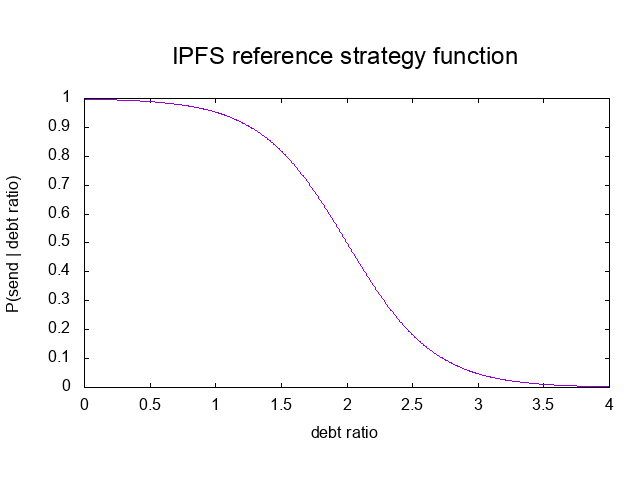
\includegraphics[width=0.7\linewidth]{img/ipfsplot}
	\caption{A plot showing the behavior of the strategy function found in the reference implementation of IPFS.}
	\label{fig:ipfsplot}
\end{figure}

A plot of this function can be found at Figure~\ref{fig:ipfsplot}. This is a type of function known as sigmoid, more specifically it is an inverted logistic function. It yields values between 0 and 1, being close to 1 with input of 0 or below, and rapidly decreasing towards 0 as the input increases.
It's easy to infer that nodes will be able to obtain blocks from a node towards which they have low debt or no debt at all; also, nodes that have exchanged many blocks in the past will be more tolerant of recent debt, allowing for some form of trust between long-lived well-behaved nodes that is directly proportional to the amount of bytes received from that given node.

When two nodes connect, they exchange their ledgers to verify that the information about previous block transfers matches: if it doesn't, both nodes clear all the information they have on the other node, losing both debt and trust that was accumulated before. A mismatch might also happen when a node is trying to clear its debt, so that another node is willing to transfer blocks with it as if it was a new node, therefore nodes are allowed to refuse communication and disconnect when a ledger mismatch happens, but this is not mandatory.

If the ledgers match, peers are connected and allowed to request and transfer blocks. Each block request is evaluated with the strategy function and accepted or denied accordingly: if a request is refused, the requesting node enters in an \textit{ignored} state and is no longer allowed to communicate for a specific amount of time (10 seconds in the reference implementation); this also happens if a received block fails the hash-based data verification step. After every completed and verified block transfer, both nodes update their ledgers.

If a node happens to have no blocks to share with other nodes but has some requests to make (either because none of its blocks are needed by the nodes discovered through the DHT or because it just joined IPFS with no blocks at all), it can \textit{work} for other nodes, by retrieving blocks needed by the known nodes in order to increase the trust from such nodes towards itself and allow the credit to be repaid by serving the originally needed blocks.

IPFS objects are \emph{immutable}. Since they are addressed by their hash, the contents of the objects cannot change once deployed on IPFS. This means that updates or new versions of objects will be published under a different address, even in the case of commits since new versions will be additional commit objects and have different hash. This makes it difficult to maintain, for example, a website where content could be frequently updated: a webmaster should continuously publish new IPFS links off-band to their users to make them aware of the website changes. To solve this problem, IPFS has a component called \emph{IPNS}~(\cite{benet2014ipfs}), which stands for InterPlanetary Name Space, and implements a mutable namespace where a unique path can be updated to refer to different IPFS objects. Each node has an IPNS path composed of \texttt{/ipns/}, to distinguish it from the immutable IPFS paths, followed by the identifier of the node, which is the hash of its public key. Under this path, there can only be \textit{signed objects}, a tuple composed by a standard object, its signature and the public key of the node, which can be verified by its hash contained in the path. Every type of standard object is supported, including trees and commits, allowing paths to reference child objects by name, similarly to IPFS. This mutable state cannot be stored in IPFS itself, therefore it lives in the DHT used for peer discovery.

\subsection{Analysis}\label{sec:ipfsanalysis}

Everything in IPFS suggests that it is meant to be deployed in a Byzantine environment. Every transferred block is verified through its hash, contained in the address, rendering impossible to counterfeit the content of the requested data; moreover, nodes that attempt to do so are detected and penalized by BitSwap through a timeout penalty.

As for the danger of free riding, BitSwap incentivizes nodes to share blocks by introducing a ledger mechanism that, while being based on the \textit{tit-for-tat} like algorithm of BitTorrent, has been made more robust through the required synchronization of ledgers between nodes: this allows to build trust among well-behaved nodes while maintaining a harsh environment for fresh nodes that join the network or towards nodes that refuse to maintain a ledger, possibly to cancel debts towards other nodes.

IPFS has an issue which is very similar to BitTorrent: just like torrent files must be distributed out-of-band, in IPFS the paths (which include the hashes) of the data must also be distributed out-of-band. But if we consider the current Web, we find the same issue: URLs of websites have to be obtained out-of-band, and the users that connect to a bad URL will not visit the webpage that they were looking for. This has been mitigated by the introduction of search engines, that made discovery of websites possible by keyword and not by URL. If a search engine behaves properly, it will return the correct URLs for the searched services. Some of these have grown to be so popular that they have started to become integrated in browsers, so that a user doesn't need to know the URL of the search engine in the first place. But the problem is only mitigated, not resolved, which allows for attacks such as \textit{typosquatting} and \textit{homograph attacks} (defined in Section~\ref{sec:squatting}).
IPFS actually improves over the Web by not being vulnerable to both of these attacks, since URLs are hashes with a strict selection of characters and a typo is almost certainly making the hash a dead link that has no associated object, but an adversary can still deliver a malicious IPFS path to a user and claim that such link leads to some content, while in reality it does not, for example by using scam e-mails or by hosting a standard website in the normal Web. IPFS also makes it more difficult for users to detect such attacks, because its paths are neither human friendly nor related to the content in a semantic way; in other words a path towards a service is not going to contain the name of that service, while in the Web it's very likely that the URL is purposefully chosen to include the service name.

IPFS uses a DHT as their peer discovery system. Any node that joins the network has to bootstrap the DHT: while IPFS does not mandate any method for doing so, the reference implementation has a list of nodes coded directly into the application from which the client bootstraps the system. Since the addresses of those nodes are well-known (they are coded in an open source application), powerful attackers can impede access to these nodes by using the censoring techniques described in Section~\ref{sec:problems}, rendering a client unable to reach the entire IPFS network. This problem has been reported in a GitHub issue~(\cite{website:ipfsbootstrap}) in the IPFS reference implementation project page, and during its discussion some solutions were proposed, including:
\begin{itemize}
	\item using the Tor network (discussed in Section~\ref{proj:tor}) to reach bootstrapping nodes in case of client-side censorship (IP blocking);
	\item reusing nodes contacted in previous sessions instead of always relying on the bootstrap list;
	\item adding a command to obtain a list of nodes from other sources, including local files, Tor, or even the BitTorrent DHT.
\end{itemize}
A temporary workaround would be to edit the list in the source code to include also more, lesser-known trusted nodes: since IPFS is open source, this is an entirely viable option.

\section{Other solutions}\label{sec:storageprojects}

Many projects that are interesting and innovative from a scientific point of view have been excluded from this thesis because they do not meet the requirements specified in the Thesis Structure in Section~\ref{sec:structure}. We will list here the most important ones, their main characteristics and the motivation behind this choice:
\begin{itemize}
	\item \textbf{Ethereum Swarm}\footnote{Ethereum Swarm: \url{https://github.com/ethersphere/swarm}}: while it features similar properties as IPFS, such as content-addressing, it is based on the Ethereum blockchain and it caters to Ethereum specific needs, such as hosting of distributed applications (or \textit{dapps}). It focuses on fast delivery of small amounts of data and really strong anti-censorship features such as \textit{plausible deniability} of ownership of data, which makes impossible to determine with certainty which node is hosting which content. At the time of writing, development is in early proof-of-concept stages with only a test network available to users.
	\item \textbf{Filecoin}\footnote{Filecoin: \url{https://filecoin.io/}}: developed by Protocol Labs and based on their own IPFS, it introduces methods to verify that data is not only stored correctly but also kept for a large amount of time, ready to be served. These methods are called \textit{Proof-of-Replication} and \textit{Proof-of-Spacetime}. Its goal is slightly different from offering a new decentralized Web (it is also suitable for personal cloud storage needs since data can be encrypted by the uploader, but without encryption it can be used to build decentralized apps). It has not been deployed at the time of writing, without even a test network available.
	\item \textbf{Dat}\footnote{Dat protocol whitepaper repository: \url{https://github.com/datprotocol/whitepaper}}: a dataset synchronization protocol designed to replicate and transfer large sets of data between peers, based on Merkle trees and public key cryptography for data verification and a DHT for peer discovery. It's the technology at the foundation of Beaker Browser, which we mention in Section~\ref{sec:browserprojects}.
	\item \textbf{Sia}\footnote{Sia: \url{https://sia.tech/}} and \textbf{Storj}\footnote{Storj: \url{https://storj.io/}}: two projects similar to Filecoin but simpler in nature. Their explicit goal is to provide a new decentralized cloud-storage service that is cheaper than the centralized ones available on the Web today.
\end{itemize}

\section{Summary}\label{sec:storagesummary}

We have explored two solutions to distribute storage of data among a number of devices in a Byzantine environment.

Both BitTorrent and IPFS rely on cryptographic hashing to verify the transmitted data: the hash information is distributed off-band in the form of torrent files and paths, respectively. Since IPFS leverages a Merkle DAG, the hash data needed to verify files is much lower in size than in BitTorrent: in IPFS only one single hash is needed, independently from the size of the data (the only variable is the hashing algorithm used to compute the hash), which allows the system to fit the hash directly into paths and to use them to address data; on the other hand, size of torrent files depends on both the block size and the overall number of blocks, but with opposing effects: torrent file size is inversely proportional to the block size but directly proportional to the number of blocks. In some cases, torrent files can reach an order of magnitude of a hundred kilobytes in size, while IPFS hashing information is in the order of tens of bytes.

The included incentive system for the protocols is different, since IPFS revisits the BitTorrent mechanism and improves on it. The algorithm based on \textit{tit-for-tat} implemented in BitTorrent does not successfully prevent free-riding, as we discussed in Section~\ref{sec:btanalysis}, a problem that IPFS attempts to solve with BitSwap, which introduces ledgers and strategies. At the time of writing it is too early to say with confidence that the current implementation correctly prevents free-riding, but BitSwap allows for different ledgers and strategies to be used (even at the same time) which enables flexible evolution of the reference implementation and the introduction of novel, more secure incentive schemes.

Both BitTorrent and IPFS rely on a DHT to perform peer discovery, but IPFS, being more recent, expands on the features of BitTorrent's DHT to achieve improved performance and fault tolerance. Neither system defines a way to bootstrap the DHT, which leaves this task to client implementers: here, BitTorrent has an advantage since many clients with different solutions exist, while IPFS has had less time to attract developers into creating their own clients, especially considering the fact that development on the reference implementation is not completed at the time of writing, forcing its developers to adopt a hopefully temporary solution by hard-coding a list of known nodes: we discuss this in Section~\ref{sec:ipfsanalysis}.

In Table~\ref{table:storagecomparison} we summarize the algorithms and mechanisms chosen by BitTorrent and IPFS to implement their solutions.

\begin{table}[h]
	\begin{center}
		\begin{tabular}{|l|l|l|} \hline
			\textbf{Feature} & \textbf{BitTorrent} & \textbf{IPFS} \\ \hline
			
			Data verification & Off-band cryptographic hashes &
			\begin{tabular}{@{}l@{}}
				Off-band cryptographic hashes \\
				Merkle DAG
			\end{tabular} \\ \hline
			
			Peer discovery & Tracker servers, DHT & DHT \\ \hline
			
			Incentive scheme & Based on \textit{tit-for-tat} & 
			\begin{tabular}{@{}l@{}}
				BitSwap strategy\\
				Reference impl. is based on \textit{debt ratio}
			\end{tabular} \\ \hline
		\end{tabular}
	\end{center}
	\caption{Summary of algorithms and techniques used by the presented distributed storage projects}
	\label{table:storagecomparison}
\end{table}

\chapter{Decentralizing Naming}\label{ch:naming}

In the Web, websites are identified by Uniform Resource Locators, or URLs, which support a very important feature: \textit{domain names}.
Domain names are strings composed by words and dots that are easy for humans to understand and memorize: the reason that we need such names is that otherwise we would have to use IP addresses in URLs which have none of those properties. Since the Internet still needs IP addresses to locate servers and devices in general, we need a system that can translate from names to IP addresses: this is accomplished by the Domain Name System (DNS).

\section{Domain Name System}

The DNS is a decentralized naming system for devices connected to a network (including the Internet), originally defined in RFC 1034~(\cite{rfc:1034}) and RFC 1035~(\cite{rfc:1035}) and updated with successive RFCs throughout the years. The most important duty of the DNS is to map arbitrary human-friendly names to mainly IP addresses, although it can map to other types of data.

The DNS defines three components:
\begin{itemize}
	\item The \emph{domain name space} is a tree data structure, where nodes are identified by \emph{labels}: labels compose the domain names in a hierarchical way, by concatenation of labels separated by dots. For example, for the domain ``\texttt{www.example.com}'', ``\texttt{example.com}'' is a child of ``\texttt{com}'' and ``\texttt{www.example.com}'' is a child of ``\texttt{example.com}''.
	\item \emph{Name servers} are programs which store information about a subset of the domain space and references to other name servers which have information about the rest of the tree. Name servers have \emph{authority} over the parts of the tree of which they have complete information.
	\item \emph{Resolvers} are programs which receive queries from clients and respond with information extracted from the name servers. Resolvers only need to know directly just one name server to complete all possible queries: if that name server does not contain the requested information, the resolver uses its references to reach other name servers.
\end{itemize}
The domain name space has one root node, labeled with an empty string. Children of this node are called \emph{top-level domains} (TLD), among which we can find ``\texttt{.com}'', ``\texttt{.org}'' and two lettered TLDs known as \emph{country codes}, such as ``\texttt{.ch}'' and ``\texttt{.it}''. As of April 2018, there are about one thousand five hundred different top-level domains (\cite{website:tldlist}).

When resolving a hostname, resolvers query the root name server with the whole domain. The root name server usually replies with the address of the name server which has authority over the top-level domain of the hostname, but it also has facility to reply with the address of the actual server associated with the whole hostname. If the query has not been completed, the query is repeated with the correspondent top-level domain name server, and so on.

To reduce traffic towards the root name servers (and all other name servers), DNS resolvers implement a \emph{caching} system: results from name servers are stored for reuse, together with an optional time-to-live value specified from the name servers themselves.

\subsection{DNS Security Extensions}

As we stated in Section~\ref{sec:problems}, DNS is susceptible to attacks, including in its caching mechanism: since it is based on UDP, it is substantially easy to forge valid packets, especially responses. The two types of messages that are most often forged are:
\begin{enumerate}
	\item Responses to resolver queries: when a browser (or any application) attempts a DNS resolution, it contacts the DNS resolver that is configured in the operating system, which is most often the one provided by the ISP, but can also be configured by the user to be any DNS resolver. If an attacker is in the proper position and quick enough, it can send a valid response before the actual resolver can get its message to the requester, causing improper data to be accepted by the application. In the case of a browser trying to find a website, it will connect to the server specified by the attacker instead of the correct one, while still displaying the original domain name in the address bar.
	\item Caching messages: a malicious name server that has authority over a domain might provide answers that are valid responses but contain invalid data, such as claims of authority over other unrelated domains or resolutions that are not competent to that name server; such data can be cached by resolvers to be used in the future, compromising access to the actual valid data.
\end{enumerate}

To counter these and similar attacks (described in~\cite{rfc:3833}), DNS Security Extensions (DNSSEC) have been introduced, which allow for resolvers and name servers to sign their messages using public-key cryptography to ensure that they originate from their actual source. Yet, implementation of DNSSEC has been inconsistent, and the majority of domains still don't support these extensions, at the time of writing.

While DNSSEC can prevent tampering of communications from a third-party attacker, it does not prevent other types of misconduct perpetrated by the DNS resolvers and name servers themselves, since they are still able to provide misleading information or to completely omit data regarding domain names that effectively become censored. This is because, from the client's point of view, DNS appears to be a centralized system (it is also a client/server protocol): the client only communicates with a DNS resolver, which will then search for the answer to the client's requests as described previously, if it doesn't already have that information.

This discussion is very similar to what is explained at the beginning of Chapter~\ref{ch:storage}. Indeed, if we consider in which failure model both the DNS and the communication channel are set, we would argue that they both lie in a stopping failure model. The usage of public-key cryptography with DNSSEC (a system parallel to HTTPS) prevents messages from being tampered with (a possibility in the Byzantine model), but does not prevent misbehavior of the DNS resolvers themselves.

To include these types of attack in our model, we would have to consider (at least) the DNS resolvers inside a Byzantine failure model, where they are allowed to omit or modify information.

\subsection{Domain squatting}\label{sec:squatting}

DNS is also vulnerable to attacks more closely related to the names themselves rather than the centralized nature of the system: \emph{domain squatting}, \emph{typosquatting} and \emph{homograph attacks}.

Domain squatting occurs when an attacker obtains a name that fully matches the name of a business or of another service, before these parties obtain that name for themselves. Thus, a user that wants to access the service or the business' website by directly typing their name into the address bar, will instead land on the attacker's website. While DNS suffers this problem, but some countries have laws in place to prevent such behavior from occurring.

Typosquatting is very similar to normal squatting, but instead of reserving the correct name, the attacker obtains a very similar name, so that if a user makes a mistake in typing the name on the keyboard (such an error is commonly referred to as a \emph{typo}), that user will obtain the attacker's website instead of being presented with an error message. DNS does not prevent this as well, and many typosquatting websites are present on the normal Web, as reported by~\cite{website:typosquatting}.

Homograph attacks, instead, do not rely on typos but on maliciously placed links: the name obtained is visually similar if not identical to the attacked name, but the characters used are not from the ASCII set, but instead use the full Unicode character map, which contains glyphs similar or identical to the ones in the ASCII set but with a different byte value associated to it. Such Unicode characters are needed to support internationalized domain names, to avoid restricting users with different alphabets than the Latin one. Users would not be able to tell the difference between the original name and the look-alike, and would click on links that seem legitimate but instead lead to an attacker's website. DNS leaves full Unicode support up to the authorities of single top level domains, therefore some TLDs support Unicode and others don't. Also, if a browser detects a mixture of character sets in a domain name it will display that URL with a technique known as \emph{Punycode}, described in RFC 3492 (\cite{rfc:3492}), that shows multi-byte characters as strings of ASCII text instead of their Unicode glyph. 

\subsection{Zooko's Triangle}

A potential solution to the Byzantine name resolution problem could be to decentralize the system, but this was thought to be impossible by~\cite{wilcox2003names}, who conjectured that one cannot obtain a namespace where names can simultaneously be:
\begin{itemize}
	\item \textbf{decentralized}: no central authority has control over all names;
	\item \textbf{secure}: an attacker cannot fake name resolutions;
	\item \textbf{human-meaningful}: names are understandable and memorable for humans, and not a randomly-looking string of text.
\end{itemize}

This \textit{trilemma} would be known as the ``Zooko's Triangle''. While decentralized namespaces already existed, they failed to either be human-meaningful (since they relied on cryptographic hashes or public keys), or to be secure (such as DNSSEC, that cannot protect against failed DNS resolvers).

This conjecture sparked discussion and interest about the problem. The birth and popularization of Bitcoin and the blockchain gave~\cite{swartz2011names} the idea that the validity of Zooko's Triangle's had been challenged by this practical and deployed project: his idea was later implemented as Namecoin.

\section{Namecoin}\label{proj:namecoin}

Namecoin is a ``key-value pair registration and transfer system''~(\cite{namecoin}) that is based on the Bitcoin blockchain. The key-value directory offered by Namecoin is mainly used to register and lookup \texttt{.bit} domains, but it can also serve other purposes, including support for ZeroNet, a project described in Section~\ref{proj:zeronet}.

At the time of writing, there is neither official documentation nor a first-party whitepaper describing Namecoin's design. The information reported here is based on either the official website~(\cite{namecoin}) or an empirical analysis by~\cite{kalodner2015empirical}.

\subsection{Protocol overview}\label{sec:namecoindesc}
Namecoin's software is a fork of the Bitcoin client: it maintains all of the features of Bitcoin with some additions, but it relies on a completely new blockchain, independent to the original one.

The Bitcoin blockchain supports the execution of non-Turing complete scripts; Namecoin in particular also defines \emph{records}, which are key-value pairs, and three additional \emph{operations} that are exclusive to Namecoin and define what functions are available to their users:
\begin{enumerate}
	\item \texttt{NAME\_NEW}: the block contains a salted hash of a name that is intended to be registered (names are used as keys in the namespace): this allows a user to publish its intention to reserve a name without actually revealing the name itself;
	\item \texttt{NAME\_FIRSTUPDATE}: the record contains the actual name that is being registered and the associated data, which can optionally include an IP address, identity information or custom data used for other services (including ZeroNet); this type of operation can be registered on the blockchain only if there is a distance of at least 12 blocks from its corresponding \texttt{NAME\_NEW} operation, and since Namecoin takes 10 minutes on average to produce a block, the wait time between reservation and reveal amounts to about 2 hours;
	\item \texttt{NAME\_UPDATE}: this operation allows for updating, renewing and trading of existing names; the type of data contained in the record is identical to the one in \texttt{NAME\_FIRSTUPDATE}.
\end{enumerate}

In Namecoin, a registered name becomes invalid (expires) after 36'000 blocks from the latest update block, including the one that contains the \texttt{NAME\_FIRSTUPDATE} operation.

To register a name there is a fee of 0.01 Namecoin: these coins are not given to any address, instead they are spent and are no longer available in the network (this operation is known as \emph{burning} coins). Also, all three of the mentioned operations cost a smaller, variable fee that is given to the user that finalizes the corresponding block, just like in Bitcoin.

On the other hand, name resolutions in Namecoin are free of charge: since the blockchain and every record contained in it is public, every device can read it and perform name lookups, even without participating in the network by verifying transactions or performing modifying operations. But in order to know the blockchain state and thus perform name resolutions autonomously, a device has to download the entire blockchain, which at the time of writing is 5.4 GB in size: this can be unfeasible for mobile devices such as smartphones and definitely out of reach for storage-restricted computers such as modems and routers. To solve this issue, some services offer name lookups through a Web-based API and others have deployed custom DNS resolvers that use the blockchain to perform resolutions but respond using the DNS protocol. Both of these solutions somewhat defeat the purpose of having a decentralized system, but improve accessibility to the Namecoin blockchain.

Records in Namecoin are JSON objects encoded in UTF-8 that can be up to 520 bytes large. The content of records mostly depends on which type of name is being registered, since Namecoin not only supports domain names (their key starts with the prefix \texttt{d/}) but also other types of names for different purposes, such as a public personal information record (with prefix \texttt{id/}), although we are only interested in domain names here.

Some of the most important keys used in domain name records (\cite{website:namecoindomainwiki}) are:
\begin{itemize}
	\item \texttt{ip} specifies the IP address associated with that domain name (\texttt{ip6} is used for IPv6 addresses), equivalently to the \texttt{A} DNS record type (and \texttt{AAAA} for IPv6);
	\item \texttt{service} is used to indicate what types of services does the associated IP provide, similarly to the DNS \texttt{SRV} record type;
	\item \texttt{alias} specifies that this name is an alias for another domain, similarly to the \texttt{CNAME} DNS record type;
	\item \texttt{email} contains the e-mail address of the registrar/webmaster, similar to the \texttt{SOA} or \texttt{RP} DNS records;
	\item \texttt{tor} specifies a hidden service domain name usable in the Tor network, which exemplifies one of the goals of Namecoin, which is to provide mappings for different types of services, including ones that may not be based on the IP network;
	\item \texttt{tls} contains TLS certificate fingerprints, allowing to specify for which protocols and ports they are used.
\end{itemize}

\subsection{Analysis}
Let's consider Zooko's Triangle applied to Namecoin and verify that this solution effectively implements all three characteristics deemed impossible to co-exist: decentralization, security and human-meaningful names.

The first and probably most trivial one is decentralization: since Namecoin relies on a blockchain to store names and associated data, and due to the decentralized, trustless nature of the blockchain, we can easily claim that there is no central authority that has control over name registration; instead, the Namecoin community collects name registrations from individuals and produces blocks that are verified by that same community and included in the blockchain, updating its state for all users of the network. Namecoin is decentralized.

Another trivial property is human-meaningful names, which Namecoin definitely supports: users are free to choose the name to register instead of having to rely on computer-generated hashes or other mechanisms that produce seemingly random strings. The purchased names are stored in the blockchain as-is (after a 12 block reservation phase in which only the hash is registered) and are shared among all nodes that maintain a valid copy of the blockchain.

The most important property and the most difficult to achieve is security. This is because, like most other characteristics, Namecoin entirely depends on the underlying blockchain, which has a probabilistic system to provide security. While some attacks are possible that would compromise the security of the blockchain (some of which derive from Bitcoin and extend to Namecoin since the design of the blockchain is really similar; more modern cryptocurrencies resolve some of these issues), the practicality of such attacks is extremely low. For example, an attack on the Bitcoin blockchain that allows \emph{double spending} (i.e. reverting a previous expense through replacement of the associated block to allow a new spending of the same coins) requires that the attacker has at least the same computing power as the sum of the power of every other Bitcoin user in the network, thus the name \emph{majority attack}, or \emph{51\% attack}. This attack has been successfully executed against other, smaller cryptocurrencies (some examples have been reported by \cite{website:realwordmajorityattacks}), which confirms that in and of itself the blockchain is not as secure as a centralized system, but the years that both the Bitcoin and Namecoin cryptocurrency have spent in operational state have demonstrated that their blockchain is secure \emph{enough} to withstand real-world attacks. Also, majority attacks are not viable in our reference model (described in Section~\ref{sec:model}) since it constrains Byzantine nodes by limiting their computing power and to a number of failed nodes below one third of the network size.

So Zooko's Triangle can be considered resolved under our assumptions. But this doesn't imply that the Namecoin system is perfect and we need to consider other attacks that go beyond the successful implementation of distributed registration and lookup of arbitrary names.

Namecoin prevents stealing of names by implementing name registration in two steps: \texttt{NAME\_NEW} is the first step, which only includes a salted hash of the name, and \texttt{NAME\_FIRSTUPDATE} which exposes both the name and the salt used in hashing. Namecoin requires that there are at least 12 blocks between the two operations: this is to avoid that an attacker reads the name on the \texttt{NAME\_FIRSTUPDATE} operation and reverts the blockchain up to where the corresponding \texttt{NAME\_NEW} was issued, then proposes a new branch of the blockchain that contain the same operations but appearing to be issued by the wrong user, thus stealing the name. The more blocks pass between the two operations, the less likely this attack can succeed, since more blocks need to be resolved by the attacker alone while the rest of the network works on the legitimate chain.

Namecoin does not have any mechanism in place to either prevent or correct \emph{domain squatting}, which appears to be very present, as described in the work of ~\cite{kalodner2015empirical}. Because of this, also \emph{typosquatting} and \emph{homograph attacks} are viable. While Namecoin uses Punycode to encode internationalized domain names into the blockchain, this does not prevent any type of attack as clients are very likely to decode names from Punycode before displaying them.

\section{Ethereum Name Service}\label{proj:ens}

Ethereum Name Service (ENS) is a name resolution system implemented on top of the Ethereum blockchain~(\cite{wood2014ethereum}). It allows name registration and mapping towards different network resources and it was first proposed as Ethereum Improvement Proposal 137 (\cite{eip:137}).

\subsection{Protocol overview}

The Ethereum blockchain supports the execution of Turing-complete scripts (called \emph{smart contracts}) that run on the Ethereum Virtual Machine (EVM). The EVM is a specification of a virtual machine that is to be executed (or emulated) by all Ethereum nodes. The EVM state is derived from all the transactions stored in Ethereum's blockchain, so that it can be synchronized among the entire network. ENS is implemented as a collection of Ethereum smart contracts and is currently deployed on the Ethereum \textit{mainnet}, its ``production'' blockchain.

ENS domain names are identical to the ones used by DNS to support potential interoperability between the two services: they are 64-bytes long labels separated by dots, that cannot surpass 255 characters in total length. ENS also takes advantage of the hierarchical nature of the domains and uses \texttt{.eth} as its only top level domain.

In ENS, domain names are encoded using a function called \emph{namehash} (\cite{eip:137}), which computes a hash using the Keccak algorithm\footnote{This is the hash algorithm used ubiquitously in Ethereum, sometimes referred to as Keccak-256 because of the 256-bit output for the specific configuration of Keccak used. Although the Ethereum documentation and its Solidity programming language refer to this algorithm as \texttt{sha3}, the actual SHA-3 standard was finalized after Ethereum was deployed and differs slightly from the Keccak-256 algorithm.}~(\cite{bertoni2009keccak}) of every label in the domain name (as defined by DNS) and then combines them together using Keccak into a single hash: this is defined as a \emph{node}, and is the only reference used by ENS to handle domains. Their readable form is never used directly in any contract, and therefore never appears on the blockchain (with the exception of reverse resolution; we discuss this later).

ENS is divided into three components:
\begin{itemize}
	\item the \emph{registrars}, smart contracts that own domains and can issue subdomains for users following the rules and fees of the smart contract corresponding to the parent domain; 
	\item the \emph{resolvers}, smart contracts that are responsible for translating names into the associated records, such as Ethereum address or hashes for content in Ethereum Swarm (mentioned in Section~\ref{sec:storageprojects});
	\item the \emph{registry}, consisting of a single smart contract that keeps track of all domains and subdomains: with each domain (specifically its node), the registry associates the owner's address, the resolver's address and the caching time-to-live for that domain and all its records.
\end{itemize}

In the current implementation of ENS, the main registrar contract (as described by~\cite{eip:ensregistrar}) is considered temporary and to be replaced approximately 2 years later since its deployment, dated 10 March 2017. This contract is responsible for domain registration (at least for domains directly under the \texttt{.eth} top level domain) and is based on an auction system. Users that want to register a name have to compete in what is described as a \emph{Vickrey auction}: users submit bids whose monetary value is kept secret from other participants and the winner of the auction pays the price of the second highest bid instead of his bid; this is done to incentivize users to bid the real amount they want to spend. The bidding period lasts three days from the start of the auction, which can be initiated by any user on any available name. After three days, follow two days called the \emph{reveal} period, in which users reveal their bid to the public: the winner obtains ownership of the domain and locks the corresponding amount in a dedicated contract called the \emph{Deed} contract, while all other participants get their bid amount back; the registry is updated accordingly. If there is only one bid, a nominal fee of 0.01 Ether is claimed from the winner. The bids contain neither the name to register nor the node for that domain, instead they contain a Keccak hash of the label that is the child of the domain for which the registrar is responsible, which is \texttt{.eth} for the main registrar described here.

The owner of a name has the right to register a resolver for its domain. Resolvers are smart contracts that must conform to a set of specific interfaces, in order to be used by automated systems or services. The obligatory method that every resolver must implement is called \texttt{has}, which can tell whether a given node and the requested record type is supported by the resolver. For each record type there are methods that allow setting and retrieval of such records for different nodes; for security reasons, only by the owner of the node can associate records with that node. Currently, the documented record types and the corresponding interfaces are:
\begin{itemize}
	\item \texttt{addr}, for resolving to an Ethereum address, which can either correspond to a contract or a wallet;
	\item \texttt{name}, for reverse resolutions back to a plaintext domain name, defined in EIP 181~(\cite{eip:181}), which allows address owners to register an authoritative name for their address (since everyone can point a name to an address by registering that name, even if its address does not belong to the name owner);
	\item \texttt{ABI}, for storing contract interfaces, which in Ethereum are usually distributed out-of-band but are essential to interact with most contracts; this is in discussion to be approved as EIP 205~(\cite{eip:205}) at the time of writing.
\end{itemize}

The public resolver contract deployed on the Ethereum mainnet (\cite{enspublicresolver}) also supports \texttt{content} records, used to handle content-based hashes like the ones found in Ethereum Swarm, \texttt{pubkey} records, which store elliptic-curve cryptography public keys, and \texttt{text} record, which simply store some textual data.

In ENS resolver contracts, all methods that perform node resolution are marked as \texttt{constant}: this indicates that those methods will not alter the state of the blockchain, which in turn means that all clients can execute these methods on their own for no fee, provided that they have access to a copy of the Ethereum blockchain, either by downloading it or through another client.

The ENS registry is very simple and straightforward. It keeps a mapping from nodes to a tuple containing the address of the owner, the address of the resolver's contract and a time-to-live value that is mostly there for DNS interoperability. Registrars communicate with the registry to update records and to verify ownerships, and the resolvers only need to talk to the registry to verify ownerships.

The ENS system is owned by seven people involved in ENS or in the Ethereum community. This allows for changes such as introduction of a new top-level domain or to recover from vulnerabilities in the currently deployed contracts, but, this effectively makes these seven people owners of every domain in the registry, allowing for changes in every record. The ownership is eventually going to be replaced by a contract and to better define governance of root nodes, making the current solution temporary.

\subsection{Analysis}

Similarly to the analysis of Namecoin, let's consider Zooko's Triangle applied to ENS and verify that the three characteristics, decentralization, security and human-meaningful names, are satisfied.

We begin with decentralization. ENS is implemented and runs on Ethereum, which is a blockchain-based system, which is in nature decentralized. Calls to smart contract functions are represented as transactions that are collected and verified in blocks by the Ethereum users: these blocks compose the blockchain, which is replicated and synchronized by all clients. But we need to consider the fact that ENS is owned by a group of seven people: while the community considers these people trustworthy, they still have effective control over every single record present in the ENS system. Therefore, even if this is a temporary solution, we can't rely on future plans or promises and claim that at the time of writing ENS is fully decentralized.

As for human-meaningful names, we can easily claim that they are supported by ENS: even though domains are handled through nodes instead of their readable form, users can directly derive nodes from domains and clients are likely to perform this transformation without the user's knowledge. For example, a potential ENS-enabled browser would most certainly accept domain names in their readable form and then compute the namehash to interact with ENS and perform resolutions; users would see, use and remember human-meaningful domain names, with a similar experience to the current Web.

Similarly to Namecoin, ENS relies on the security of the underlying Ethereum blockchain. As Bitcoin, Ethereum is vulnerable to majority attacks, but they are unlikely to occur in the current real-world settings and not feasible in our reference model described in Section~\ref{sec:model}.
We should also consider failures from the deployed ENS smart contracts, possibly deriving from bugs or issues in the implementation that have not been discovered yet: this is one of the reasons that led to assigning ownership of the ENS system to a group of seven trustworthy people in the Ethereum community, so that if any problem arises with the contracts themselves or with the system those people can intervene and potentially fix the implementation bugs and/or recover from loss or unauthorized alteration of records. While this fact by itself does not inherently guarantee security, it is an additional measure to counter potential incidents or attacks.

We now move our attention to more general naming concerns, starting with name stealing. ENS successfully prevents this attack by implementing a \emph{Vickrey auction}: bids happen independently from one another over a three day time span and are followed by two more days in which bids can only be revealed. Once a bid is revealed, no other user can place a higher bid on that name, therefore it is safe to reveal bids. Also, if one would want to revert the blockchain back to undo both the reveal and the bid and replace them with their own, it would need to revert and propose potentially several thousand blocks: Ethereum's target block time is 15 seconds, which means that the network will most likely produce more than 5'000 blocks per day. If the bid and its reveal are distant enough (some hours should suffice), this attack becomes unfeasible under our model assumptions.

ENS does not have mechanisms in place to prevent \emph{domain squatting} and the related attacks, \emph{typosquatting} and \emph{homograph attacks}. We can consider the fact that the ``centralized'' ownership of ENS allows for interventions to resolve situations where such attacks were enacted, but it seems unlikely that this would be done at the current stage, knowing that the deployed registrar is considered temporary. We also have to note that in the ENS FAQ document~(\cite{website:ensfaq}) it's stated that the next permanent registrar will aim to provide fairness (``The system should not unduly favor people who happen to be in the right place at the right time'') and to implement a principle of least surprise (``Wherever possible, names should resolve to the resource most users would expect it to resolve to''), so this is likely to impact feasibility of these attacks, but this is not part of the current registrar.

\section{Other solutions}
ENS supersedes other previous attempts to implement DNS-like functionality on the Ethereum blockchain: such projects were either simpler in nature or did not allow different types of records to be registered~(\cite{eip:137}), so it would be redundant to include them here.

Other projects not related to Ethereum are:
\begin{itemize}
	\item \textbf{EmerDNS}\footnote{EmerDNS: \url{https://emercoin.com/en/documentation/blockchain-services/emerdns/emerdns-introduction}}: part of a larger blockchain-based project known as Emercoin, whose goal is to provide secure and distributed business services and operations, not to develop an alternative to the Web;
	\item \textbf{NXT Aliases}\footnote{NXT Aliases: \url{https://nxtplatform.org/what-is-nxt/alias-system/}}: part of another blockchain-based project called NXT, aliases are  generic key-value associations that allow any string to be associated with any other, possibly shorter string. Similarly to Emercoin, NXT provides many features but not a distributed Web;
	\item \textbf{Blockchain Name System}: we discuss this in Section~\ref{proj:blockstack}.
\end{itemize}

\section{Summary}

We have explored two solutions, Namecoin and ENS, which aim at decentralizing naming systems through replication in a Byzantine environment.
Both Namecoin and ENS rely on the blockchain, a data structure that implements Byzantine fault tolerant consensus. Both projects store names on the blockchain, which is then used to synchronize information among all participants of the network. While Namecoin uses and expands on the operations provided by Bitcoin, ENS takes advantage of Ethereum's smart contracts, which are more powerful as they are Turing complete, while Bitcoin scripting is not.
They allow ENS to provide both more capabilities, for example ENS takes advantage of domain hierarchies by introducing custom resolvers, and more structure, since record formats are enforced by the resolver smart contracts instead of being stored as JSON objects, whose content and format cannot be enforced.

Regarding Zooko's Triangle, both projects have the potential to challenge this idea by implementing a decentralized secure system for handling human-meaningful names. But, if we consider the details, we cannot claim that ENS is decentralized because of the ownership of the system by seven esteemed people in the Ethereum community, which have complete control over every single record in the system. Instead, Namecoin does not have this weakness and successfully refutes Zooko's triangle.

Both systems successfully prevent name stealing by hiding the domain name through hashing at the moment of expressing interest for it, for later revealing the clear-text name to prove the claim. Namecoin will allow only one name claim and will assign the name when it is revealed, while ENS implements a more complex auction system in which also the bid amount is hidden (known as a Vickrey auction). The time between claim and reveal also differs in the two projects, with Namecoin having a minimum wait time corresponding to verification of 12 blocks (approximately two hours) and ENS allowing up to 5 days.

None of the two systems resolves attacks such as squatting, typosquatting and homograph attacks. If we consider DNS, which by itself does not solve this problem, its centralized ownership allows for interventions by governments or other similarly powerful parties that can resolve cases in which these attacks were successful. ENS technically allows this as well by having the owners of the system intervene in case such attacks were enacted, but there is no actual mechanism in place that prevents the attacks from succeeding. Namecoin on the other hand can neither prevent nor recover from these attacks. It would seem like this vulnerability appears to be directly caused by assigning human-meaningful names to a free, unregulated market, which is the one the blockchain has become popular for. In such a market, it all comes down to who obtains the name first, which disregards company names, trademarks or other types of already existing recognizable names: vulnerability to the attacks are a direct consequence of this. Though, it is worth noting that ENS has plans to forbid the attacks through a smart contract that owns the ENS records: in the future we will see if the ENS teams can accomplish this and how they will manage to do so.

In Table~\ref{table:namingcomparison} we summarize the main features and accomplishments that characterize Namecoin and ENS.

\begin{table}[h]
	\begin{center}
		\begin{tabular}{|p{4.5cm}|p{3cm}|p{4.5cm}|} \hline
			\textbf{Feature} & \textbf{Namecoin} & \textbf{ENS} \\ \hline
			
			Underlying technology & 
			\begin{tabular}{@{}l@{}}
				Blockchain \\
				(Bitcoin fork) \\
			\end{tabular} &
			Blockchain (Ethereum)	\\ \hline
			
			\begin{tabular}{@{}l@{}}
				Refutation of Zooko's Triangle \\
				1. Decentralized \\
				2. Secure \\
				3. Human-meaningful names \\
			\end{tabular} &

			\begin{tabular}{@{}l@{}}
				Yes\\
				1. Yes \\
				2. Yes \\
				3. Yes \\
			\end{tabular} &

			\begin{tabular}{@{}l@{}}
				No\\
				1. No (has central ownership) \\
				2. Yes \\
				3. Yes \\
			\end{tabular} \\ \hline

			Prevention of name stealing & Yes (hashed name) & Yes (hashed name, auction) \\ \hline
			
			Prevention of squatting and related attacks & No & No (but can recover through human intervention)
			\\ \hline
		\end{tabular}
	\end{center}
	\caption{Summary of features and accomplishments of the presented distributed naming projects}
	\label{table:namingcomparison}
\end{table}


\chapter{Distributed Web Projects}\label{ch:projects}

We have previously discussed how key Web components like storage of data and naming can be realized in a Byzantine failure scenario, and we explored projects that have implemented and exemplified our descriptions. In this chapter, we see how the two components can be combined to obtain a solution that may be called the distributed Web.
Thus, the projects we're going discuss next provide a complete, Web-like, user experience, either by extending the functionalities of existing browsers or through some specific browser-like interface.

To satisfy our requirements for a distributed web (see Section~\ref{sec:problems}), these projects must satisfy the following:
\begin{itemize}
	\item Resistance to \textbf{censorship}, by using a distributed data storage system that correctly decouples websites from IP addresses and by relying on a valid peer discovery system and good incentive scheme;
	\item Lack of \textbf{trust}, by using Byzantine fault tolerant protocols to transfer data and to resolve names without the need of trusting any external party;
	\item Support for \textbf{privacy}, allowing users to fully control the data that they share and who they share it with.
\end{itemize}

\section{ZeroNet}\label{proj:zeronet}

ZeroNet is the first distributed Web project that we present. It combines BitTorrent and elliptic-curve cryptography (the same system used in Bitcoin) to provide distributed storage of data, and takes advantage of the Namecoin system to provide support for decentralized domain names.

\subsection{Project overview}

We start by defining some general concepts of the ZeroNet system. Being a peer-to-peer system, a client is called a \emph{peer}. A ZeroNet website (or \emph{zite}, as the community has grown to call them) consists of a collection of files that are listed in a special file named \texttt{content.json}. To exchange messages between peers, ZeroNet uses MessagePack~(\cite{website:msgpack}), which provides a JSON-like interface but a more compact data representation.

ZeroNet's data verification mechanism is based on the same elliptic-curve public key cryptography used in Bitcoin\footnote{This allows website owners to receive Bitcoin payments since the public key is also a valid Bitcoin address. This feature is planned to be integrated into ZeroNet, but this is not implemented at the time of writing.}: each website is identified by a public key that is also used to address it. Once a client fetches a website, the first request is to the \texttt{content.json} file, which is signed by the website creator using the corresponding private key; the client verifies the file against the website's public key. This file is essential to the data verification mechanism since it contains the SHA-512 hash of every single file of that website. The client will then download these files from the network and will be able to verify their integrity against their previously obtained and already verified hash.

ZeroNet does not really implement an incentive scheme, instead it applies a very simple rule to replicate data: peers that visit a website will also start to serve the downloaded files to other peers. The incentive that this rule is meant to provide is that popular websites that are visited by many people will be heavily replicated, ensuring a long lifespan, while unpopular, or even worse, sites that contain potentially illegal content will not be visited, especially since visitors will automatically serve those unwanted files, and no copies of that website will be made.

ZeroNet bases its peer discovery solution on BitTorrent, more specifically on BitTorrent's trackers: a client will request to a tracker which peers are currently serving a specific website and the tracker will return those peers. This action also adds the requesting peer to the list of currently serving peers. ZeroNet implements a peer exchange system equivalent to BitTorrent's PEX, in which clients can suggest the IP addresses of other peers by using a dedicated message of the protocol. ZeroNet also includes a tracker server in its code, so that any client can also function as a tracker server if configured accordingly.

Since websites are addressed by their public key, ZeroNet URLs are not human-meaningful. While this identification mechanism is sufficient to retrieve websites, ZeroNet supports Namecoin's \texttt{.bit} domain names: clients will obtain the record for the requested domain name and search for the key \texttt{zeronet} in the obtained JSON, which is expected to contain the ZeroNet public key of the corresponding website; clients will then proceed to obtain the list of peers and the website files as described above. As we stated in Section~\ref{sec:namecoindesc}, to perform resolutions in Namecoin, a client would need to download the entire Namecoin blockchain. Instead, ZeroNet relies on ZeroName, an internal ZeroNet site that stores all ZeroNet enabled domains registered on Namecoin. ZeroNet can also be configured to use a locally running Namecoin client in case the user wants to perform resolution against the actual blockchain.

The ZeroNet client is not a browser, thus it is not able to render websites on its own. Instead, the client starts an HTTP server on port 43110: the way that this server is meant to be accessed is by pointing existing browsers towards that server and to pass, through the URL, information on which website the ZeroNet client needs to retrieve. This is the reason behind the unique format of ZeroNet URLs: they all start with \texttt{http://127.0.0.1:43110/}, since this would be the address of the Web server run by the ZeroNet client when run in the same computer in which the browser is making the requests. The element that follows the URL identifies the website, either by its public key or by a ZeroNet enabled Namecoin domain. The rest of the path specifies which file to load. If the path is empty, the browser is redirected to ZeroHello, a ZeroNet website that is meant to serve as a ``homepage'' for the network.

It is worth noting that the ZeroNet client does not simply relay content from the network to the browser, instead it provides a more complex Web interface that allows features such as displaying a loading page while the website is retrieved, or \emph{real-time website updates}. This last feature uses WebSocket API to let the interface know that content on the page has changed and that new data has to be displayed accordingly; under the hood, the content creator's client has sent a message to some current visitors, which are then going to relay the message to other peers, that a newer \texttt{content.json} file is available. When a client is notified, it compares timestamps to verify that the file is actually newer, and then downloads the new content accordingly.

A key feature that allowed the rise of social media is the ability to get, store and serve user-generated content. ZeroNet supports this through \emph{multi-user sites}: this feature allows website owners to give other users the ability to modify specific files of the website, effectively enabling user-generated content. The key of the user that obtains editing permission is stored in a \texttt{content.json} file and the user has to sign its changes through another \texttt{content.json} file specific to this user, so that the new content can be verified not only for integrity, but also for checking that no other user is submitting content without permission.

ZeroNet is not made with anonymity as a priority and it is stated in various resources (\cite{website:zeronetpresentation}, \cite{website:zeronetfaq}) that ZeroNet is ``not more anonymous than BitTorrent'', in the sense that it is possible to identify which IP address created a website and uploaded its content into the network, and also who is currently serving files of some website. On the other hand, ZeroNet supports interoperability with Tor, an anonymizing network, so that all traffic can be routed through it without the risk of being de-anonymized by some Tor-unaware part of the system; an example of software that can de-anonymize its users is BitTorrent, as presented and analyzed by~\cite{manils2010compromising}.

\subsection{Analysis}

We start by checking if the ZeroNet data transfer protocol fits our Byzantine failure model defined in Section~\ref{ch:background}. Assuming that elliptic-curve cryptography is strong enough to resist computationally limited attackers, ZeroNet's data verification system correctly functions under our assumptions: the \texttt{content.json} file is verified against the website's address, which is either known or provided by the Byzantine fault tolerant Namecoin, to avoid tampering.

Two other characteristics of ZeroNet are sources of concern. First, the chosen incentive scheme does not help in replicating all data that is stored in the network.
This could be considered intentional and justifiable since the rationale behind this choice is to penalize content which is not worth of replication. Instead of blindly replicating all content unconditionally, the community (i.e., content popularity) decides what merits replication. Second, the peer discovery system is centralized, as it is based on BitTorrent's trackers that we already discussed in Section~\ref{proj:bittorrent}: while BitTorrent solves this by providing both a DHT and PeX as alternatives, ZeroNet only provides an equivalent to PeX, and this is not sufficient as this method is not reliable, since peers can refuse to share or provide misleading information about other peers, just like trackers. Similarly, peers can also setup their own tracker servers to be used by the rest of the community, but this has the exact same issues as peer exchange, with the added hassle of having to configure the client to contact these new trackers, instead of having the feature work out of the box.
%todo(leandro) - it's not clear to me here: does the DHT satisfy your requirements?
% It does, and ZeroNet does not have a DHT

From the above we derive that ZeroNet data transfer protocol is not Byzantine fault tolerant since peer discovery can be compromised. The lack of a BFT peer discovery system exposes ZeroNet to potential censorship as trackers and peers alike can refuse to provide correct information when requesting clients that share some given sites. On the other hand, it is worth noting that, in order to function, peer discovery only needs one non-failed tracker that provides enough information to discover a sufficiently large portion of the network, which then allows for peer exchange to be viable and improve on connectivity with other peers. But this is not enough to obtain BFT peer discovery: censorship attacks are unlikely to target only a portion of trackers, especially since a list of the servers used by ZeroNet is directly obtainable from the project's source code; since trackers are a small number of fixed servers, we argue that subverting more than 1/3 of them is feasible.

The naming system used by ZeroNet is Namecoin, which we discussed in Section~\ref{proj:namecoin}. What is of interest for us here is the way that ZeroNet uses Namecoin information: instead of contacting the blockchain directly, which would be the safest solution, naming data is obtained from the blockchain off-band and stored in the internal site ZeroName, against which the client performs name resolutions. Assuming that the off-band channel is trusted (apparently the main ZeroNet developer known as ``nofish'' has a script that updates ZeroName regularly~\cite{website:zeronameupdate}), this method is as secure (in the Zooko's Triangle sense) as performing resolutions on the blockchain directly: this is because data from the website is verified against the \texttt{content.json} file, which is itself verified against the ZeroName's public key stored in the client.
Compromises in the peer discovery system might make this website inaccessible, but do not hamper transfer of information once a valid peer is found.
This mechanism cannot be considered trustless, as we need to trust ZeroName's maintainer to provide correct naming resolution data.
The solution is to rely on an actual Namecoin client and configure ZeroNet to use that instead of ZeroName.

In ZeroNet, every information contained in websites is public. There is no mechanism in place to privatize content or to make some data available to only selected users. This makes it impossible to keep personal information secure, in fact no private or identifying information should be shared on this platform and any of its websites. 
A feature that would enable some form of private data management called ``private sites'' is planned, although development has stagnated and no progress is being made~(\cite{website:zeronetprivatesites}).

\section{Blockstack}\label{proj:blockstack}

Blockstack is a blockchain based decentralized platform that aims to provide a new, distributed internet. This network can be accessed through the first-party Blockstack Browser, available as either a normal website~(\cite{website:blockstackbrowser}) or as a downloadable client~(\cite{website:blockstackdownload}). The Blockstack system is described in a technical whitepaper by~\cite{blockstack}.

\subsection{Project overview}

The Blockstack network is divided into three layers:
\begin{enumerate}
	\item The foundation of the entire network are \emph{virtualchains}, data structures that rely on existing blockchains to store the information while providing all logic themselves;
	\item The peer network called \emph{Atlas}, which provides information on where to retrieve data;
	\item The \emph{Gaia} storage system, that allows users to store data on custom servers or on existing cloud storage providers, all through the same interface.
\end{enumerate}

Let us start by defining what is a virtualchain and how it's used in Blockstack. A virtualchain is essentially a virtual blockchain that abstracts some information away from existing blockchains and provides the capability to construct state machines on top of this abstraction. The only requirements that a virtualchain needs from a blockchain are that transactions are totally ordered (a feature that all blockchains provide) and that additional arbitrary data can be stored with transactions. Virtualchains use this extra data space to store a \emph{consensus hash}: a hash derived from both the virtualchain transactions in the current block and the consensus hashes of previous blocks. This hash is used to verify data in virtualchain blocks and to avoid accepting new transactions that either contain unknown hashes or that are based on blocks that are too old, with stale consensus hashes. Since hashes are stored in a standard blockchain, they are protected from Byzantine attackers, and thus all virtualchain data can be verified without the need of trusting anyone in the network.

Virtualchains provide a very important feature: the ability to migrate from a blockchain to another. This allows virtualchains to continue to function even after the blockchain on which the system is based is compromised. A virtualchain migration starts from announcing the block number from which that blockchain will no longer be used (this has to be an unreleased future block). Then, the state currently on the virtualchain is written to the target blockchain, and once this operation is complete, the current virtualchain users will verify that the transferred state is indeed consistent with their internal state. From here, new virtualchain blocks will be accepted on the new blockchain. Blockstack used this feature to migrate its virtualchains from Namecoin to Bitcoin~(\cite{website:blockstackmigration}).

We placed virtualchains at the foundation of the network because they are the root component that provides verification data for the rest of the elements in this system: in the whitepaper, this concept is defined as \emph{bootstrapping trust}. Blockstack uses virtualchains to implement the Blockchain Name Service (BNS).

The BNS system divides names into \emph{namespaces}, which correspond to the top-level domains in DNS. Each namespace has its own virtualchain and all namespaces are handled by a root virtualchain, which makes it possible to purchase new namespaces if some user wishes to do so. A namespace virtualchain handles name operations such as purchase, update, transfer and revocation of names. In particular, the purchase operation is very similar to Namecoin's: users first \emph{preorder} a name and then confirm it with a \emph{registration} transaction, that effectively assigns ownership of that name to the user.

Even if there is no auction to assign names, BNS purchase fees are not fixed, instead, they are based on \emph{pricing functions} that determine the price for a name based on factors such as the name itself. For example, the pricing function for the \texttt{.id} namespace will yield a lower price for long names than for short ones, and will lower the price even more if the name contains non alphanumeric characters: this is to discourage users to purchase short names (which are potentially more desirable than longer and complex ones) if they don't plan on actually using it.

To describe associations from names to records, BNS uses \emph{zone files}, which are short text files with a table-like format that define the records for that particular name. Zone files are also used in DNS to define records for a particular zone, and are the inspiration for BNS' own files, which use the same format. On the other hand, zone files are not stored directly into BNS: instead, they are stored in the Atlas network, and BNS only keeps the public key of the owner, the record keys and hashes of the record values, so that the content of zone files can be retrieved and verified in a trustless manner.

Atlas is an \emph{unstructured} peer-to-peer network. This means that there is no data structure to collect information about peers, such as a DHT: instead, each node randomly chooses a set of neighbors, thus shaping the network as a regular graph. Traversing such a graph would be difficult, therefore Blockstack developers removed this need by fully replicating the data in the network: all nodes have a complete copy of all the data.

Information in the network cannot be added without first announcing it on the BNS virtualchain, so that the data can be verified by the nodes. This effectively implements a whitelist of data allowed to join the network, which prevents flooding attacks where massive amounts of data are being uploaded into the network: such attacks would be devastating in a fully replicated setting.

Atlas zone files contain URIs that point to where the actual data is located. This data belongs to the storage system known as Gaia, which is very different from the distributed storage systems we have seen in Chapter~\ref{ch:storage}. In Gaia, storage is separated by user, or in other words, each user with a record in BNS has ownership of its own data. In fact, the user is also responsible for providing the disk space in which the owned data is to be stored: in addition to privately owned servers, Gaia supports online cloud storage providers such as Amazon S3 and Dropbox. The user chooses which service is to be used (more than one can be chosen to provide redundancy) and then stores through Gaia its files on those services. Gaia clients are responsible for handling data verification: files stored through Gaia are signed with the user's private key so that they can be later verified with the public key stored in BNS. Gaia also supports encryption of data and access-control capabilities to limit data access to some known addresses (explained in more detail in the Gaia GitHub repository:~\cite{website:gaiaaccesscontrol}).

When considering the scope of such a system, Blockstack developers put the emphasis on storage of user data (such as personal information, documents, images etc. of the users of the service) to be used in Blockstack-enabled applications and websites, rather than using the network for hosting the application data or the website itself.
In fact, they implemented storage of user data as Blockstack IDs, which are identifiers on the BNS that are connected through Atlas and Gaia to information that can be used on all Blockstack-enabled services.
Users define through Gaia where they prefer to store their data and who can see it. Applications request access to this data directly to the user through the Blockstack Browser, which acts as a client for the Blockstack network.

\subsection{Analysis}\label{sec:blockstackanalysis}

The solution proposed by the Blockstack team is really unique in its structure, especially considering the storage system Gaia. Data verification is guaranteed throughout all the sub-projects that compose the network: at the bottom, virtualchains rely on the blockchain's BFT consensus to build a trustless state machine, used to implement the Blockchain Name Service; then the Atlas network uses the BNS to verify and index all data that it contains; then, at the top, Atlas' zone files are used to locate the Gaia storage provider chosen by the name owner, whose content is verified against the name owner's public key, stored in BNS. This makes Blockstack a fully trustless system.

BNS' pricing functions provide an interesting potential solution to name squatting and related attacks: since the pricing depends on the name, a function that increases cost of potentially valuable names can discourage squatters to buy such names in the first place. The pricing function for the \texttt{.id} namespace considers short names more valuable than long names, which is a justifiable reasoning, since short names tend to be more memorable and therefore more valuable, but fails to consider actual popular names that can have a very high value, even if they are long. It would be interesting to see if a more complex function that considers real-world popularity data would be effective in preventing squatting entirely.

If we move our attention to censorship resistance, we can spot a vulnerability in Gaia's replication system: all addresses to the data associated to a name are contained in a public zone file, and all of these addresses are standard URIs, often even HTTP URLs in case of cloud storage services like Amazon S3 or Dropbox. The data is ultimately stored in a \emph{centralized} manner and is vulnerable to censorship. Even if this data can be replicated among different services, including custom servers operated by the owner itself, this does not resolve the issue as custom servers are likely to fail under a DDoS attack, while cloud storage providers are vulnerable to powerful parties such as public pressure or governments, assuming that they don't decide to remove the data themselves.

A solution to this problem would be to add support for storage providers that are decentralized and censorship resistant, since the most important information that Gaia needs is a URI coming from Atlas, so technically any storage system that supports URIs could be implemented. This has been discussed and the Blockstack team is open for contributions from the open source community to provide support for Sia, Storj and IPFS~(\cite{website:gaiaimprovements}).

The most important part of Blockstack is the focus on privacy of user data. This is directly expressed in the realization of Blockstack IDs and its surrounding API that allow developers to build applications based on it. Users have full control over their data through the Gaia system, including its location (on which service it is hosted, including personally owned servers) and which applications can access it. This data can also be shared among different services, which allows for better interoperability between applications, even if they are potential competitors (say, for example, two social media websites). Blockstack developers have also encouraged adoption of this feature by registering on BNS a \texttt{.id.blockstack} namespace where users can register a Blockstack ID without paying a fee, directly through the Blockstack Browser.

As of now, the Blockstack network is not used to directly serve websites, even if the system technically supports it. Instead, developers currently build applications that only use the network for Blockstack IDs, and not for storing and serving application data, which is instead in the form of native clients distributed through the standard Web or is made available directly as a website.
An example of this is the first-party demo application ``Hello Blockstack''\footnote{Hello Blockstack: \url{https://helloblockstack.com/}}, which is itself a standard website, but makes use of the Blockstack platform to enable user login through their Blockstack ID.

\section{Other solutions}\label{sec:browserprojects}

The development scene in the distributed web area is active, with many projects currently in early stages or still in planning phase, sparked by the current trend of blockchains and decentralization, but there are also other, older projects that were born from activism promoting freedom of speech and communication. Among all these projects, the most notable are:

\begin{itemize}
	\item \textbf{SAFE Network}\footnote{SAFE Network: \url{https://safenetwork.org/}}: a project developed by MaidSafe\footnote{MaidSafe: \url{https://maidsafe.net/}} that aims to reuse available hard disk space of computers to provide a distributed storage system, which can be accessed and explored with the SAFE browser; at the time of writing, this project is only available on an Alpha test network;
	\item \textbf{Beaker Browser}\footnote{Beaker Browser: \url{https://beakerbrowser.com/}}: based on the dataset synchronization protocol known as Dat, Beaker Browser allows for creation and visualization of distributed websites, although it fails to provide or reuse a distributed naming system, relying instead on HTTP and DNS to resolve names;
	\item \textbf{Freenet}\footnote{Freenet: \url{https://freenetproject.org/}}: a very mature project, with its initial release dating back to the year 2000, it's a peer-to-peer platform focused on anonymity and censorship resistance; Freenet allows browsing websites, known as \emph{freesites}, but the naming scheme is based on nicknames, which are simply labels defined and stored by single users and not shared globally, thus not satisfying decentralization from Zooko's Triangle.
\end{itemize}

\subsection{Alternatives to decentralization}\label{proj:tor}
If we consider the three properties that we want to achieve (censorship resistance, lack of trust and better privacy), we can't help but mention other projects that offer these characteristics without recurring to decentralization, thus not implementing a distributed Web. Instead, heavy use of encryption and redirection of traffic through multiple hops allow to \emph{anonymize} communications, possibly achieving all three of the mentioned properties. Such projects are known as \emph{anonymity networks}, of which the most popular one is Tor~(\cite{website:tor}).

Tor is a peer-to-peer network composed by nodes that act as \emph{relays} of traffic. The core mechanism of Tor, known as \emph{onion routing}, is to encrypt messages exchanged within the network as many times as the number of relays (also known as \emph{onion routers} or simply routers) through which communication happens. To accomplish this, a Tor client first establishes a \emph{circuit}, i.e. selects three ordered random nodes through which passes all communication to the rest of the Internet. It then obtains the public key of each router, and encrypts the message three times, using each time the key of the latest relay that will receive the message: for example, if the circuit is composed of routers A, B and C, the message is encrypted first with the key of C, then with B's key and then with A's key. Each time the message is encrypted for a router, the destination that the message should be delivered next is included in the packet (e.g. when encrypting for B, C's address is included with the message), so that each router (and only the single router) knows where to deliver the message.

This routing method achieves the following properties: the first router doesn't know the content of the message, nor its final destination; the second relay knows neither who the message originated from, nor the content of the message nor its final destination; the third router (also known as the \emph{exit node}) knows the content of the message and its final destination, but not who generated the message. This is done such that if any one (but only one) of the nodes is owned by a malicious attacker, this attacker does not have enough information to de-anonymize the user.

Tor also supports websites internal to the network, a type of \emph{hidden service} (the term refers to all types of services, including mail or chat servers). They can be reached by typing their address in the Tor Browser, a version of Firefox tuned to better protect users from losing their anonymity. These address are effectively domain names that use the \texttt{.onion} top level domain, but are not human-meaningful, as they are directly derived form the public key of the website.

Tor achieves censorship resistance as the IP address of users and of hidden servers is not available to the rest of the network (hidden services' address is protected through a mechanism described in~\cite{torhiddenservice}). Since the address of users and service owners is not known, standard attacks like the ones described in Section~\ref{sec:problems} are not possible without performing a de-anonymizing attack first (examples of such attacks are from~\cite{jansen2014sniper} and~\cite{kwon2015circuit}), which we will not delve into as they are outside the scope of this Section: assuming such attacks are impractical, Tor can be considered censorship resistant.

The level of trust required to utilize Tor depends on the task that a user wants to accomplish: the system is trustless when used to access hidden services, as the communication between the server and the user is end-to-end encrypted and the server's identity can be verified through its address (more details in~\cite{torhiddenservice}); on the other hand, when Tor is used to access the external Internet anonymously, users need to trust the exit node of their circuit as it can see, and potentially tamper with, the data that passes through it. A solution to this is to encrypt communication between the user and its external service through methods like HTTPS, so that the exit nodes cannot modify the data they relay without alerting the user or the service.

While Tor provides anonymity to its users, the user's data needed in the interaction with hidden services is handled in the same way as in the standard Web: the services keep user data in their servers, outside of user's control. Privacy controls are not provided by Tor, but instead the responsibility of offering such tools reside on the hidden services themselves. Not even the law here can enforce privacy regulations, as hidden services are protected from identification and therefore not accountable for their conduct.

Projects similar to Tor are the Invisible Internet Project, also known as I2P~(\cite{website:i2p}) and Freenet, already mentioned in Section~\ref{sec:browserprojects}.

\section{Summary}

We have explored two solutions that attempt to implement the distributed Web through combining or developing solutions for managing decentralized storage and naming.

The two projects, ZeroNet and Blockstack, differ in nature. ZeroNet offers more ``classical'' peer-to-peer networking, taking heavy inspiration from BitTorrent and completing its solution by relying on Namecoin, while Blockstack follows the blockchain based approach and provides an original, custom network stack by augmenting its basis with virtualchains, the Atlas network and the Gaia storage system.

If we consider censorship resistance, ZeroNet provides the better solution, even if it's not perfect: website visitors automatically copy and serve its contents, building a somewhat ``popular-first'' replication system that favors frequently visited websites over rarely accessed ones. ZeroNet's vulnerability to censorship resides in the peer discovery system, based on BitTorrent's trackers, which are a centralized entity and allows for attackers to impede access to the network or to take over and control data returned by them.
Blockstack is also vulnerable to censorship, but on the Gaia layer,
since the location of the data is static and known publicly through Atlas zone files. At the time of writing, Gaia does not support decentralized ``back-end'' storage systems that are not vulnerable to standard Web attacks, such as IPFS.

As for trust, ZeroNet technically needs to trust the trackers in order to function correctly, for the same reasons that we discussed above, but once the peer network is bootstrapped, no trust is required as all received data can be verified with the website hash, which is either known or obtained from the trustless Namecoin system. Blockstack, on the other hand, does not need trust in order to function: the blockchain ``bootstraps trust'' for the entire network, since all data contained in virtualchains, in the Atlas network and in Gaia ultimately can be verified with data contained in the blockchain. While cloud-storage providers supported by Gaia may need to be trusted to keep the data, a user can also setup a personally owned server which can act as fail-over in case said providers fail, removing the need to trust them.

When it comes to privacy the two systems provide radically opposite offerings: ZeroNet completely lacks support for privacy of data, instead every file stored in the network is public (although it plans to support ``private sites''). Blockstack, on the contrary, fully implements privacy controls, making them central to the whole system through Blockstack IDs: with Gaia, users can control where to store their data and who to share that information with; Blockstack-enabled applications have to request access to user data directly to the user, through the Blockstack Browser.

We also mentioned anonymity networks, in particular the Tor network, which provide a potential alternative to the distributed Web for resolving the issues of the current Web.

In Table~\ref{table:dwebcomparison} we summarize the main features and characteristics that ZeroNet and Blockstack exhibit. From the table, it is clear that ZeroNet does not reach our requirements for a decentralized Web, while Blockstack is more fit but still lacks some properties, especially considering how the current system is used for Blockstack IDs only, instead of also storing websites.
%todo(leandro) - what is the difference between user data and a website?
% The website is provided by the content creator, user data means everything from personal information to user generated content. I replaced user data with Blockstack IDs to make it clearer.

\begin{table}[h]
	\begin{center}
		\begin{tabular}{|p{3.5cm}|p{4.5cm}|p{4cm}|} \hline
			\textbf{Feature} & \textbf{ZeroNet} & \textbf{Blockstack} \\ \hline
			
			Underlying technology & 
			\begin{tabular}{@{}l@{}}
				Custom data transfer protocol \\
				BitTorrent trackers \\
				Namecoin \\
			\end{tabular} &
			\begin{tabular}{@{}l@{}}
				Blockchain (Bitcoin) \\
				Atlas peer network \\
				Gaia storage system \\
			\end{tabular}	\\ \hline
			
			Censorship resistance & No (uses trackers) & No (centralized storage) \\ \hline
			
			Lack of trust & No (uses trackers) & Yes \\ \hline
			
			Privacy controls & No & Yes \\ \hline
		\end{tabular}
	\end{center}
	\caption{Summary of features and characteristics of the presented distributed Web projects}
	\label{table:dwebcomparison}
\end{table}

\chapter{Conclusions}\label{ch:conclusions}

We have described the current state-of-the-art for the decentralized Web. We first have defined a Byzantine failure model that more appropriately represents the reality of the Web and its vulnerabilities. We then have shown that BitTorrent and IPFS provide a feasible solution for storing and distributing data in such a model, with even more projects such as Filecoin and Ethereum Swarm potentially launching in the future. We then moved our attention to implementing human-meaningful naming in such a model, presenting Namecoin and ENS as currently viable solutions. Then, we defined the distributed Web as the combination of decentralized storage and naming and explored two projects that satisfy our definition: ZeroNet and Blockstack. We also presented Tor, an alternative to content decentralization which provides censorship resistance through onion routing.

Development of the decentralized Web is in its early stages. New projects and solutions continue to arise, making this area very dynamic and full of innovation. Events such as the Decentralized Web Summit~(\cite{website:dws}) are gaining popularity and traction, hosting informative talks and making the scene more interconnected by having members of different organizations talk to each other and confront ideas. This document is bound to become obsolete within the next years as more projects evolve and reach stable deployment, but it is still interesting to explore the current technologies since they create the foundation for what is next to come.

It's also worth stating that none of the projects described here have become massively popular among Internet users as alternatives to the standard Web. The most popular one, BitTorrent, is well known for its file sharing capabilities instead of being part of ZeroNet's data transfer system.

\section{Future work}

In this work we have highlighted flaws that affect some of the projects described. Since many of these projects are open source, contributions to their development to fix their issues represent potential future work of this thesis. For example, we mentioned in Section~\ref{sec:blockstackanalysis} that Blockstack needs developers that can implement IPFS support in Gaia; many other projects also welcome open source contributions.

A project that requires much work but has great potential of implementing a distributed Web is Ethereum, through combination of Ethereum Swarm and ENS. Supporting development of these features also classifies as future work of this thesis.

%todo(leandro) - not critical, but I though of this question: is there some specific problem which is currently not well addressed by the current solutions?
% Nothing that applies to more than one project comes to mind.

Among the projects described we cannot identify a system that fully satisfies our vision of the distributed Web. Possible future work would be to develop new projects that combine features from existing systems or implement novel techniques to bring original and valuable improvements over the systems described here.

%\appendix

\backmatter

\bibliographystyle{alpha}
% \bibliographystyle{dcu}
% \bibliographystyle{plainnat}
\bibliography{webrbiblio}

%\cleardoublepage
%\theindex %optional, use only if you have an index, must use
	  %\makeindex in the preamble
%\lipsum

\end{document}
